\documentclass[12pt]{scrartcl}

%\usepackage{subfiles}
\usepackage{amsmath}
\usepackage{scrextend}
\usepackage{titling}
\usepackage{setspace}
\usepackage{graphicx}
\usepackage{caption}
\usepackage[export]{adjustbox} %for right alignment of gigure
\usepackage{wrapfig}
\usepackage{tikz}
\usetikzlibrary{shapes.geometric,arrows}

%-----------------------------------------------------
\renewcommand{\abstractname}{\centerline{\textbf{Abstract}}}
\newcommand{\blankline}{\hfill\break}
\graphicspath{{./figures/}}
\renewcommand*\descriptionlabel[1]{\hspace\leftmargin$#1$} %for where discriptions of equations http://tex.stackexchange.com/questions/36500/how-to-provide-a-definition-for-symbols-in-a-latex-math-equation
\tikzstyle{startstop} = [rectangle, rounded corners, minimum width = 3cm, minimum height = 1cm, text centered, draw=black, text width=5cm, fill=red!30]
\tikzstyle{io} = [trapezium, trapezium left angle=70, trapezium right angle=110, minimum width=3cm, minimum height=1cm, text centered,trapezium stretches=true,  draw=black, text width=10cm, fill=blue!30]
\tikzstyle{process} = [rectangle, minimum width=3cm, minimum height=1cm, text centered, draw=black, text width=10cm, fill=orange!30]
\tikzstyle{decision} = [diamond, minimum width=3cm, minimum height=1cm, text centered, draw=black, text width=10cm, fill=green!30]
\tikzstyle{arrow} = [thick,->,>=stealth]
%------------------------------------------------------
\title{PHASOR: A Exit Wave Phase Reconstruction Code in MATLAB\textsuperscript{\textregistered}}
\author{Amit Gupta\\{Supervised by: Prof. S. Vasudevan}\\Dept. of Inorganic and Physical Chem.\\Indian Institute of Science\\\texttt{amit@ipc.iisc.ernet.in}}
\date{}

\onehalfspacing

\begin{document}
    \bibliographystyle{unsrt}
    {\Huge{\maketitle}}
    \newpage
    %!TEX root = ./main.tex
\begin{abstract}
    \abstractname
    \blankline
    %\bibliography{references}
    Electron microscopy was was first developed by Ernst Ruska in year 1956.
    Ever since its conception, electron microscopy has provided valuable insights into our world.
    It has now become one of the most powerful and versatile tool at scientists' disposal. 
    However as we know, electron microscopy uses electromagnetic lenses, which are highly aberrated.
    This results in image degradation and causes loss of lots of valuable information. 
    This problem has been solved almost completely by aberration corrected electron microscopes, which are however still considerably costly.

    Another problem routinely encountered by microscopes originate from the physics of image formation.
    Whenever an image is formed any information related to `phase' of scattering sample is lost.
    This information of phase is important for several reasons, most importantly it results in higher resolution as well as gives us information about sample thickness and elemental composition.

    Out of many methods suggested to recover this phase information and to remove effects of aberrations, one of the simplest is exit wave reconstruction. 
    It is simple to implement and highly effective.
    In following pages we would discuss fundamentals of imaging physics and exit wave reconstruction using Inverse Weiner Filter method, followed by detailed discussion of a simple exit wave reconstruction code written in MATLAB\textsuperscript{\textregistered}.

    Exit wave of electron microscope consists of symmetric and anti-symmetric part.
    We shall limit the discussion and implementation to symmetric part of exit wave only.
    The Inverse Weiner Filter method, among other concepts used here were already published in literature.\cite{meyer_symmetric,meyer_unsymmetric}
    \end{abstract}
    %!TEX root = ./main.tex
\section{Introduction}

\subsection{A brief overview of Phase Contrast}
\begin{wrapfigure}{L}{0.45\textwidth}
    %\begin{figure}[!b]
        \centering
       % \begin{minipage}{0.6\textwidth}
            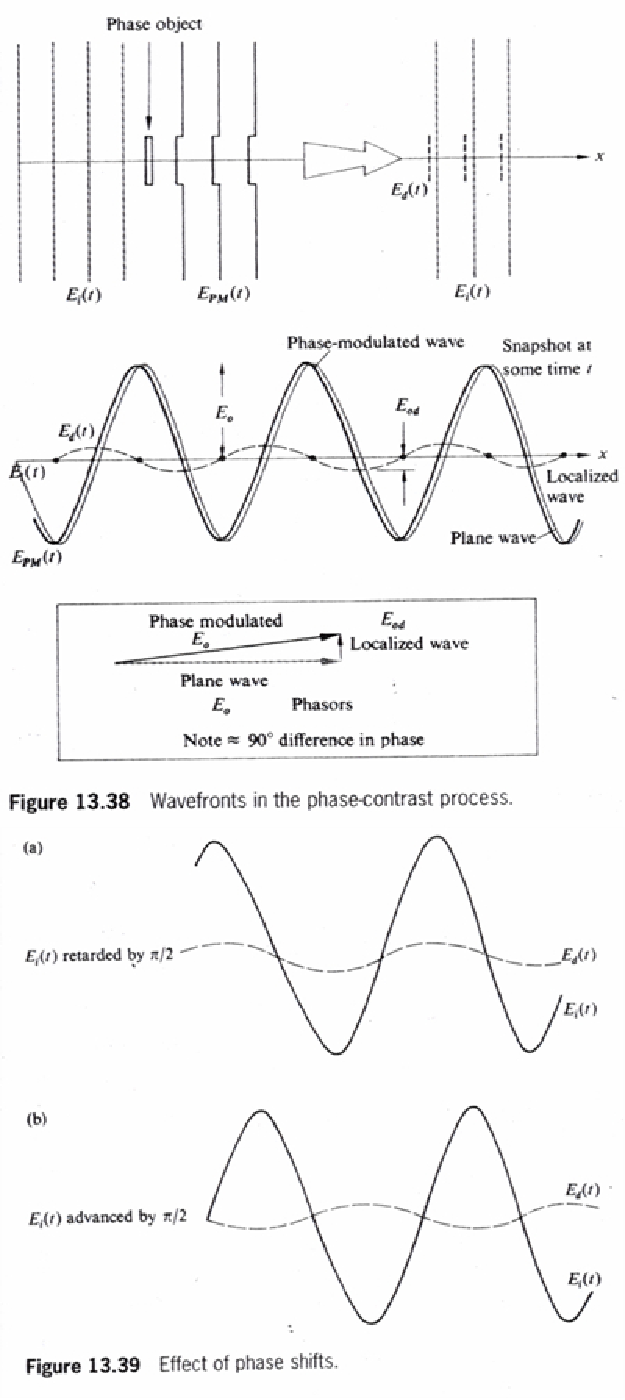
\includegraphics[width=0.45\textwidth]{figures/phasediff.pdf}
            %\captionsetup{margin={0pt,0.6\textwidth},width=\textwidth}
            \caption{Wavefronts in phase contrast process (image credit `Optics by Eugene Hetch')}
            \label{fig:hetchphase}
       % \end{minipage}
    %\end{figure}
\end{wrapfigure}


Phase contrast microscopy has been around for quite a while.
While it has revolutionized the world of optical microscopy, it also provided interesting insights into physics of imaging in itself.
Whenever any nearly `transparent' object scatters any incoming wave, it leaves the amplitude of the wave more or less intact, however phase of the incoming wave is altered very slightly.
This small advancement or retardation of phase results in difference of $\pi/2$ between the 2 waves(Figure~\ref{fig:hetchphase}).
Usually this phase difference will not make any noticeable change in contrast, but if incident or scattered wave is modulated by extra phase of $\pi/2$. then this phase contrast can be converted to amplitude contrast.
This is the fundamental principle behind phase contrast microscopy.

There is another method to extract information of phase from the image object, that is `holography'. 
Basic idea behind holograhpy is to record an interferogram between scattered wave and incident wave, this way all of the information of original scattering object is retained in single interferogram or hologram.
Holography, for our interest here, can be divided in roughly 2 segments:
\textbf{Inline} and \textbf{Off-axis} holography.
Inline holograhpy was first described by D. Gabor in 1948.\cite{Gabor1948}.
In Inline holography, scattered waves from an object interfere with unscattered waves from the same source to produce hologram.
While in Off-axis holography, incoming beam is first split into two beams, one of which then interacts with the object, after which it interferes back with the other half (the unscattered wave) to produce the hologram.

\begin{wrapfigure}{L}{0.5\textwidth}
    \centering
    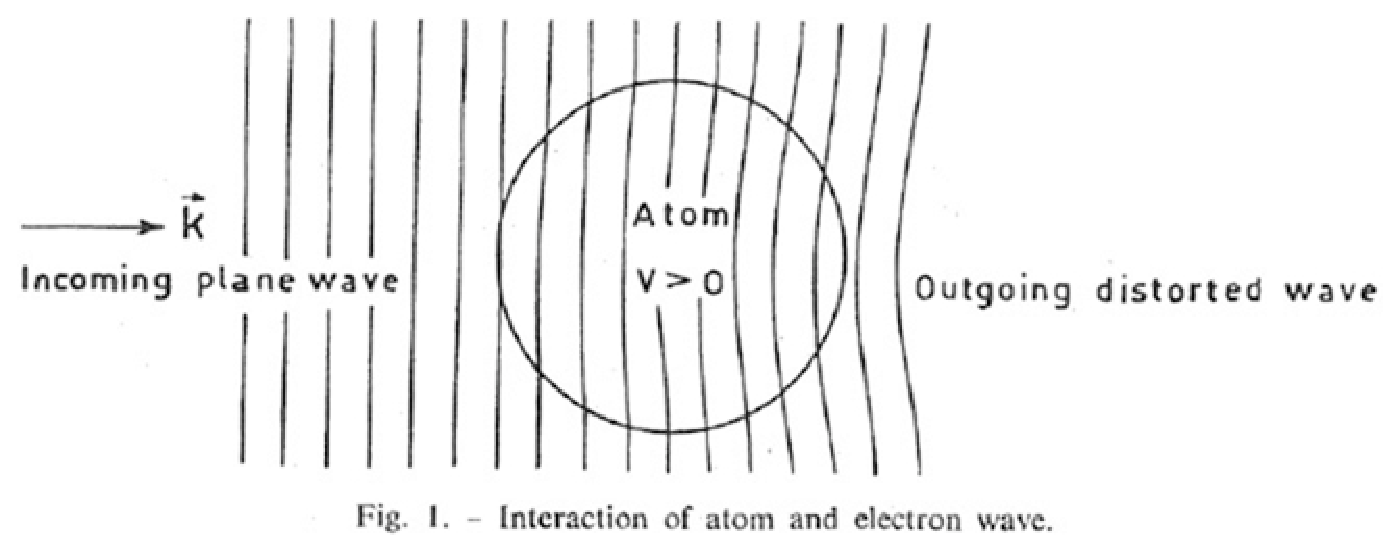
\includegraphics[width=0.5\textwidth]{figures/electronphase.pdf}
    \caption{Electron plane wave retardation by an atom (image credit: unknown)}
    \label{fig:electronphase}
\end{wrapfigure}

The high resolution electron microgram, produced from highly coherent field emission source, is an inline hologram.
Hence it not only contains information about the position of particles but their relative phases as well.
When an electron plane wave passes through an atom, due to the positive potential at the core atom, phase of electron waves advances slightly (Figure~\ref{fig:electronphase}).
Hence now the distorted electron plane wave carry information about not only position of atoms (relative phases with respect to each other), but also of atomic number of the atom (magnitude of phase change).
This information if extracted can elucidate entire structure of any given sample.
This as formed image of the sample on the plane wave of electron is called `Exit Wave'.

Problem for electron microscopy is complicated slightly by the lens aberrations.
As we shall see shortly phase of electron plane wave in an electron microscope depend on the defocus value and aberration coefficients of the electron microscope.
Hence to reconstruct our original object we have to deconvolute effects of both defocus and aberrations from our images to obtain pure exit wave.
To understand effects of aberrations on the image, first we need to have a look at the transfer function of electron microscope.


\subsection{Effects of Defocus and Spherical Aberration}
We shall discuss effects of two defects in image which do not originate from sample ($k$-spacing) or from physical limitations of electron beam (\textit{e.g.} decoherence and $\lambda$), \textit{i.e.} defocus and spherical aberration.

\begin{figure}
    \centering
    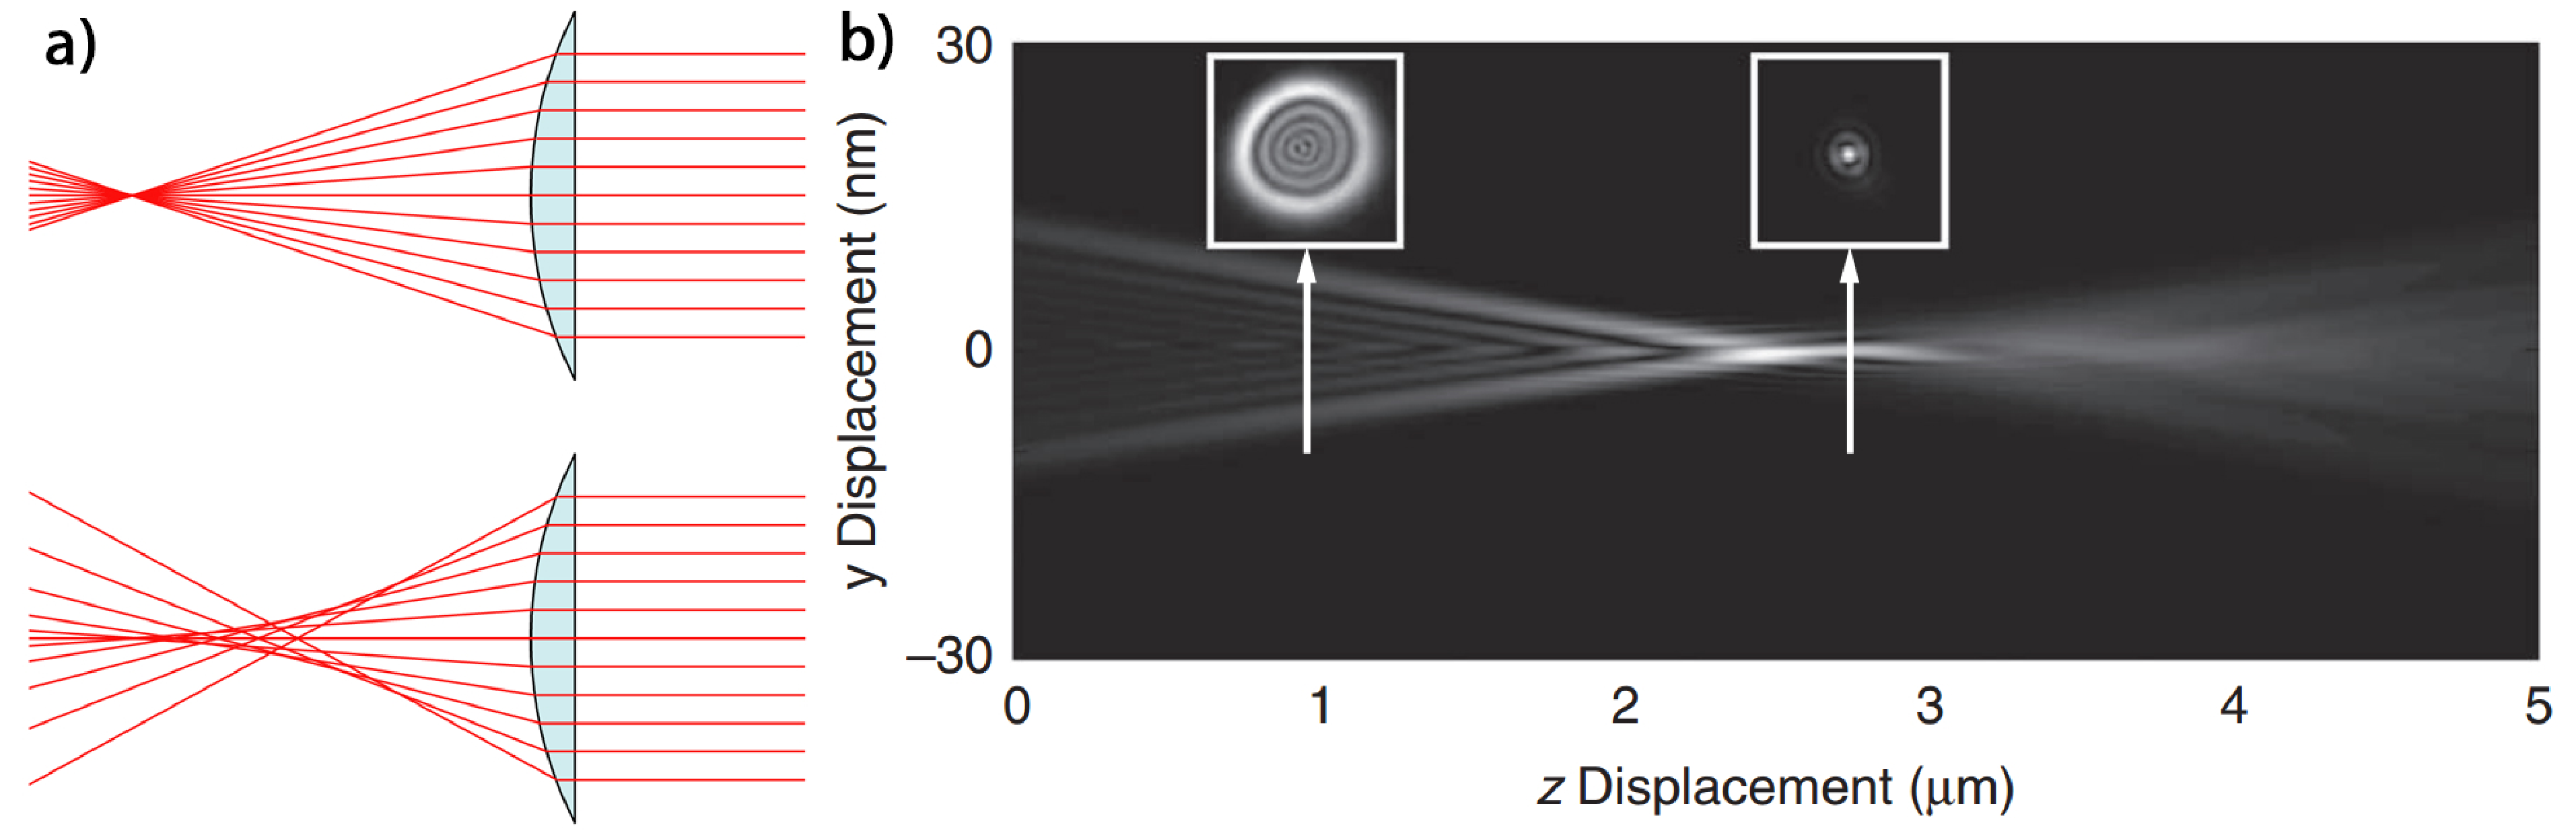
\includegraphics[width=\textwidth]{figures/circleleastconf.pdf}
    \caption{a) Simple diagram showing perfect lens with point focus and lens with spherical aberration, and b) Probe size at different defocus values for a source focused with lens having spherical aberration (Ref \cite{Humphry2012})}
    \label{fig:leastconfusion}
\end{figure}

\textbf{Defocus} is simply defined as the difference between the plane in which currently lens is focusing as opposed to the plane in which lens shall focus ideally.
Focal length of lens is essentially the point where image of a point is reproduced as a point.
Any lens with any defect in it will not reproduce image of a point as a point but rather as `spread', whose precise form is determined by the Point Spread Function (PSF) of the lens.
If a lens has no other defect but just defocus, then its PSF can be described mathematically as a simple Gaussian function.


\textbf{Spherical Aberration:} Spherical aberration is the defect in optics when rays, coming from different part of of lens (from the edge of the lens as compared to near axis of lens) focuses at different positions long principal axis, as shown in Figure~\ref{fig:leastconfusion}a (when it focus at same value of principal axis but at different positions in plane $\bot$ to lens plane, then it is called `Coma').
Because of spherical aberration PSF of a point is now rather represented as a disk.
The smallest of such disk which is created by spherical aberration is called `Circle of Least Confusion', as that is sharpest image that could be produced of a point (Figure~\ref{fig:leastconfusion}b).
As pointed out by Scherzer\cite{Scherzer1949}, due to cylindrical symmetry of EM lenses and the fact that EM lenses can only be converging, (magnetic field is always stronger at edges as compared to the center of lens hence it can only converge the electron beam) all EM lenses contains inherent spherical aberration (in optics spherical aberration is corrected by diverging lenses to compensate for the difference in focal lengths).
\footnote{For correcting spherical aberration, lenses were needed which were not cylindrically symmetric. Among other ideas such as lenses with charged axis etc, multipolar lenses were suggested (see \cite{Rose2009} for detailed discussion).
In 1997 first successful practical aberration corrected TEM was reported using hexapole correctors \cite{Haider1998}, followed by an independent report using quadrapole/octapole correctors \cite{Batson2002}.
Aberration correction by the use of multipole unsymmetrical lenses will not be discussed any further.}

In fourier optics, as discussed earlier image formation can be described as the convolution of PSF of the lens on to the perfect image of object  to be imaged.
In case of TEM it would be convolution of PSF of objective lens on to the exit wave of sample.
Point spread function of TEM is rather complex and is discussed in detail in following section.


\subsection{Contrast Transfer Function}
Transfer functions are described as mathematical functions of and `response' given from any instrument. 
That is, as in the case of TEM, the function mapping the outgoing exit wave (electron lane wave after interacting with the sample) to the observed contrast or image.
As image formation is done by objective lens, in above case it will be the transfer function of the objective lens, \textit{i.e.}
\begin{equation}
    \psi_t(x) = t(x) \psi_{inc}(x)
    \label{eq:exitwave1}
\end{equation}

where: 
\begin{description}
    \item[\psi_{inc}(x)] = incident plane wave
    \item[t(x)] = transmission function (ie how, for different `x', $\psi_{inc}(x)$ is modified after transmission from sample)
    \item[\psi_t(x)] = exit plane wave, i.e electron plane wave just after passing through the specimen
\end{description}

Effects of lens aberrations on $\psi_{t}(x)$ is to shift intensity of it as a function of aberrations and spatial frequency (lattice spacing of various planes).
Effects of such aberrations can be represented mathematically as the convolution operator.

\begin{equation}
    \psi_i(x) = \psi_t(x) \ast h_o(x)
    \label{eq:imgplnconv}
\end{equation}

where:
\begin{description}
    \item[\psi_i(x)] = image plane wave
    \item[\ast] denotes convolution operator
\end{description}  

In fourier space it can be written as:
\begin{align*}
    FT\{\psi_i(x) = \psi_t(x) \ast h_o(x)\}
\end{align*}
\begin{equation}
    \Psi_i(\boldsymbol{k}) = \Psi_t(\boldsymbol{k}) . H_o(\boldsymbol{k})
    \label{eq:fourierconv}
\end{equation}
That is because, convolution operator in real space is multiplication in fourier space.
Here $H_o(\boldsymbol{k})$ can be described as:
\begin{equation}
    H_o(\boldsymbol{k}) = exp(-i\chi(\boldsymbol{k}))
\end{equation}
where $\chi(\boldsymbol{k})$ is `Wave Aberration Function' which can be described as:
\begin{equation}
    \chi = 0.5 \pi C_s k^4 \lambda^3 + \pi \Delta f k^2 \lambda + \pi \Delta f_a cos(2(\theta - \theta_c)) k^2 \lambda + \textnormal{higher order terms}... 
\end{equation}

Here:
\begin{description}
    \item[C_s] = Spherical aberration coefficient of the Objective lens
    \item[\Delta f] = average defocus
    \item[\Delta f_a] = variation in defocus due to 2-fold astigmatism
    \item[\theta_c] = angle of astigmatism w.r.t x-axis
\end{description}

Higher order terms include aberrations such as three fold astigmatism, coma, and higher order spherical aberration etc.
For non-aberration corrected TEMs $C_s$ and two fold astigmatism overwhelms other aberrations, hence they shall be focus for now.
Higher order aberrations does show noticeable image degradation in aberration corrected TEMs.

According to weak phase approximation\cite{Scherzer1949}, sample is so thin that it does not affect the amplitude of the electron beam, rather only shifts its phase.
This approximation is valid depending upon 2 things mainly i) sample thickness and ii) atomic number of sample.
While weak phase approximation may remain true for C film for over few nanometers easily, a single uranium atom can invalidate the assumptions.
If weak phase approximation is held true then only above phase difference will be the contrast contributing member HRTEM images.
In such case only complex part of $H_o(\boldsymbol{k})$ is of any interest.
Hence, neglecting higher order terms, and assuming sample to be weak phase object, transfer function can simply be written as $sin$ function or:
\begin{equation}
    T(k) = -sin(\frac{\pi}{2}C_s \lambda^3 k^4 + \pi \Delta f \lambda k^2)
    \label{eq:ctf}
\end{equation}

Therefore it can be stated that information represented in TEM image is controlled by two factors, namely i) Spherical aberration ($C_s$) and ii) defocus ($\Delta f$)
Besides $C_s$, coherency of beam also affects the transfer function of the TEM.
Spatial decoherence of electron plane wave results in formation of an envelope function which reduces contrast at higher spatial frequencies.
Envelope function for coherence ($E_c$) can be represented as :
\begin{equation}
    E_c = e^{|\nabla\chi|^2\beta^2/(4\lambda^2)} e^{-\pi^2\lambda^2d^2 k^4/2}
    \label{eq:chromatic}
\end{equation}
Here:
\begin{description}
    \item[\beta] = convergence angle of beam
    \item[d] = defocus spread due to chromatic aberration 
\end{description}
Contrast Transfer Function or CTF of TEM can now be described as the product of the actual transfer function (Equation~\ref{eq:ctf}) and envelope function (Equation~\ref{eq:chromatic}).
Here the value at which CTF converges to zero is call Information Limit of the microscope.
\begin{figure}[t]
    \centering
    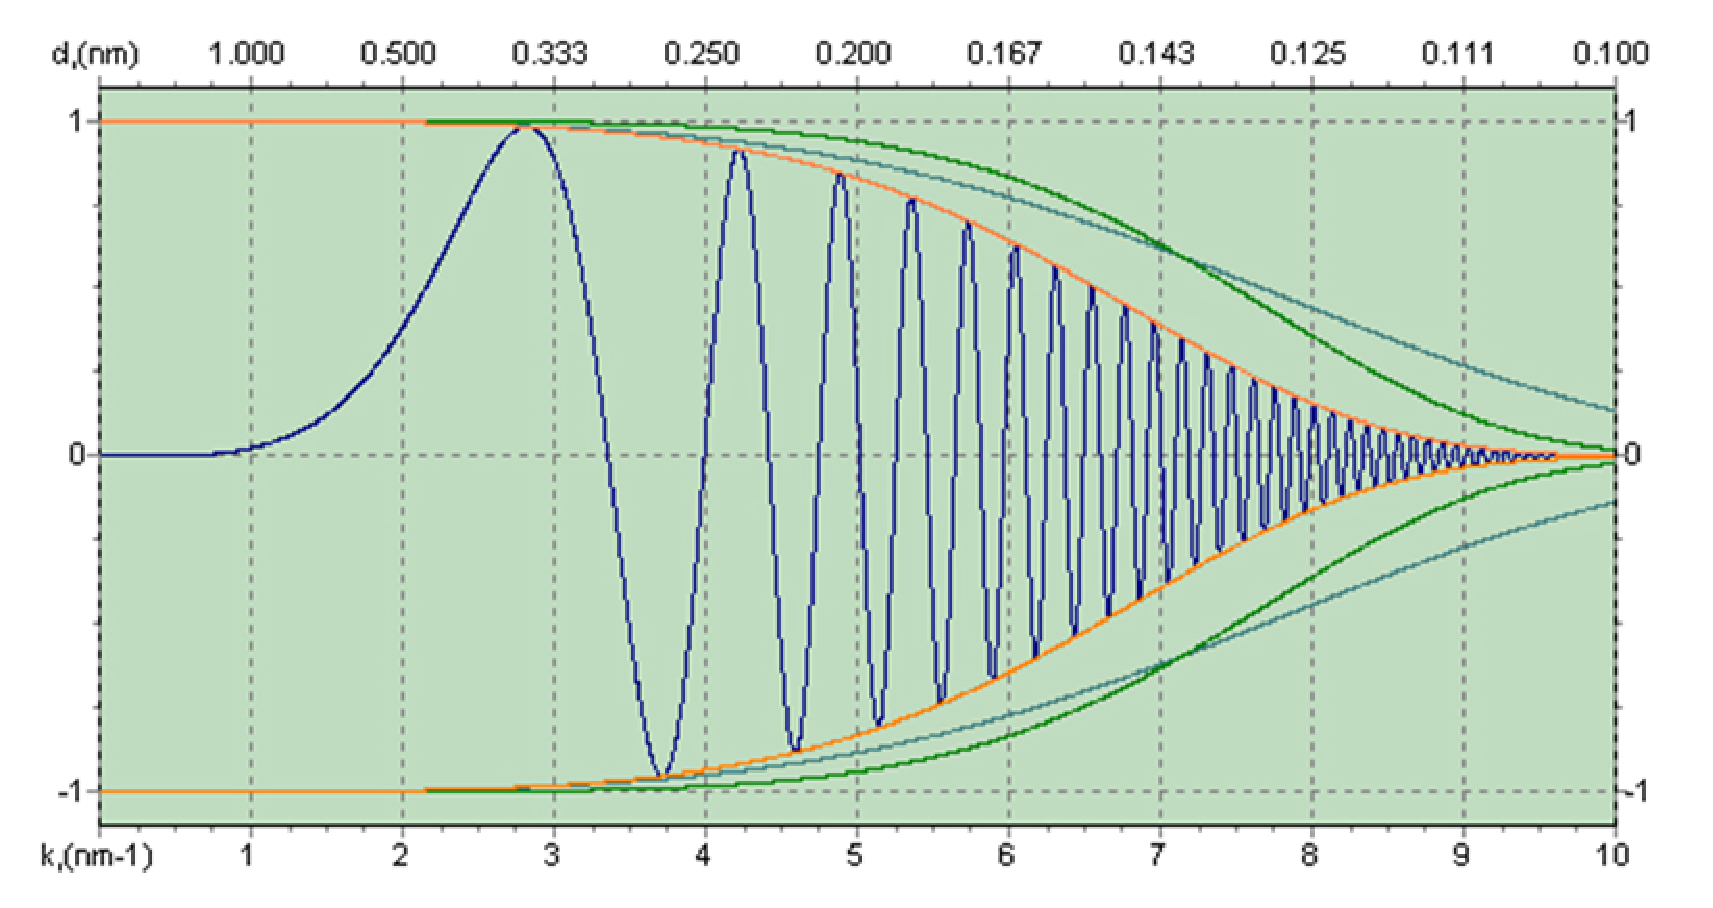
\includegraphics[width=0.8\textwidth]{figures/ctf.pdf}
    \caption{Contrast Transfer Function of TEM (Blue), orange line represents the envelope function}
    \label{fig:ctffigure}
\end{figure}


\begin{wrapfigure}{L}{0.45\textwidth}
    \centering
        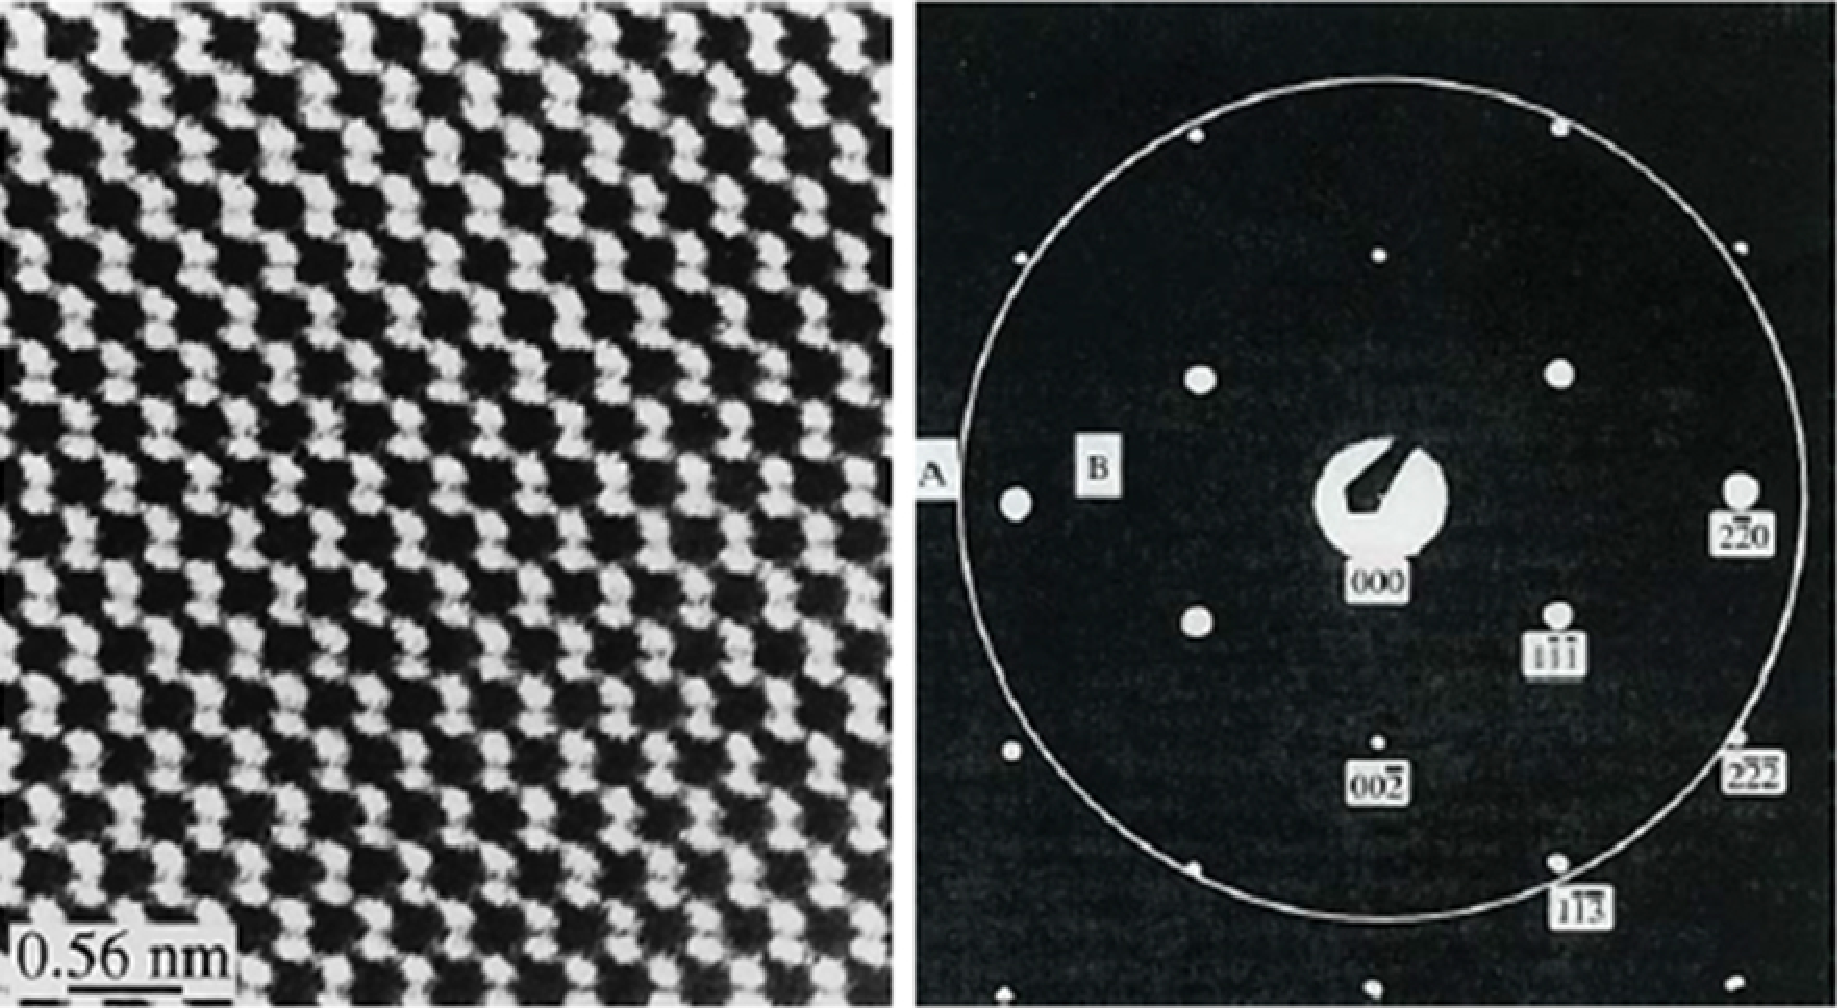
\includegraphics[width=0.45\textwidth]{figures/siwrong.pdf}
        \caption{HRTEM image showing Si `dumbbells' which were mistakenly  identified as from $d_{004}$ lattice}
        \label{fig:siwrong}
\end{wrapfigure}


Figure~\ref{fig:ctffigure} shows CTF vs $k$ plot.
As it is evident, CTF for TEM is not linear but sinusoidal.
Hence depending upon the lattice spacing, in any given image, some lattice planes might appear dark while others might appear light or may not appear at all (zero transfer of contrast).

This makes direct interpretation of HRTEM images rather difficult because TEM image is now complex interference pattern of various lattice spacings of varying intensity. 
At this point any attempt to find position of any atoms present or any direct measurement of lattice constants etc can be severely misguiding.

Shown here in Figure~\ref{fig:siwrong} is one such TEM image where the appearance of `dumbbells' in Si HRTEM was identified as atoms from $d_{004}$ lattice fringes.
Actual fringe spacing of Si $d_{004}$ is 0.14nm and measured $d$-spacing was 0.013nm, leading to the confusion.
It shall be noted that not only microscope resolution limit was much lower, 0.25nm, but at time of image capture objective aperture was masking the $d_{004}$ spot (shown Figure~\ref{fig:siwrong} diffraction pattern with a white ring).
Ultimately that dumbbells were assigned to interference pattern from $d_{113}$ fringes.
This illustrates the difficulties and pitfalls in directly correlating HRTEM intensities with spatial positions of atoms.\footnote{It is often repeated advice that in HRTEM image is forming from interference of various lattice spaces, hence they do not represent true position of atomic columns. An interesting take against this advice can be read here [https://publications.lbl.gov/islandora/object/ir\%3A122777/datastream/PDF/view] by Prof Micheal A. O'Keefe. 

There author mainly discusses how under correct conditions intensities on TEM image does indicate presence of atomic columns, hence incorrect imaging conditions shall not be the reason to say the above statement about atomic positions.}


Other than variation in intensities as described above, spherical aberration also degrades images in one more way, it is called threading.
As spherical aberration focuses electrons nearer to edge of lens more, electron which are scattered the most, with higher $k$ value or low $d$-spacing are focused first.
\begin{figure}
    \centering
    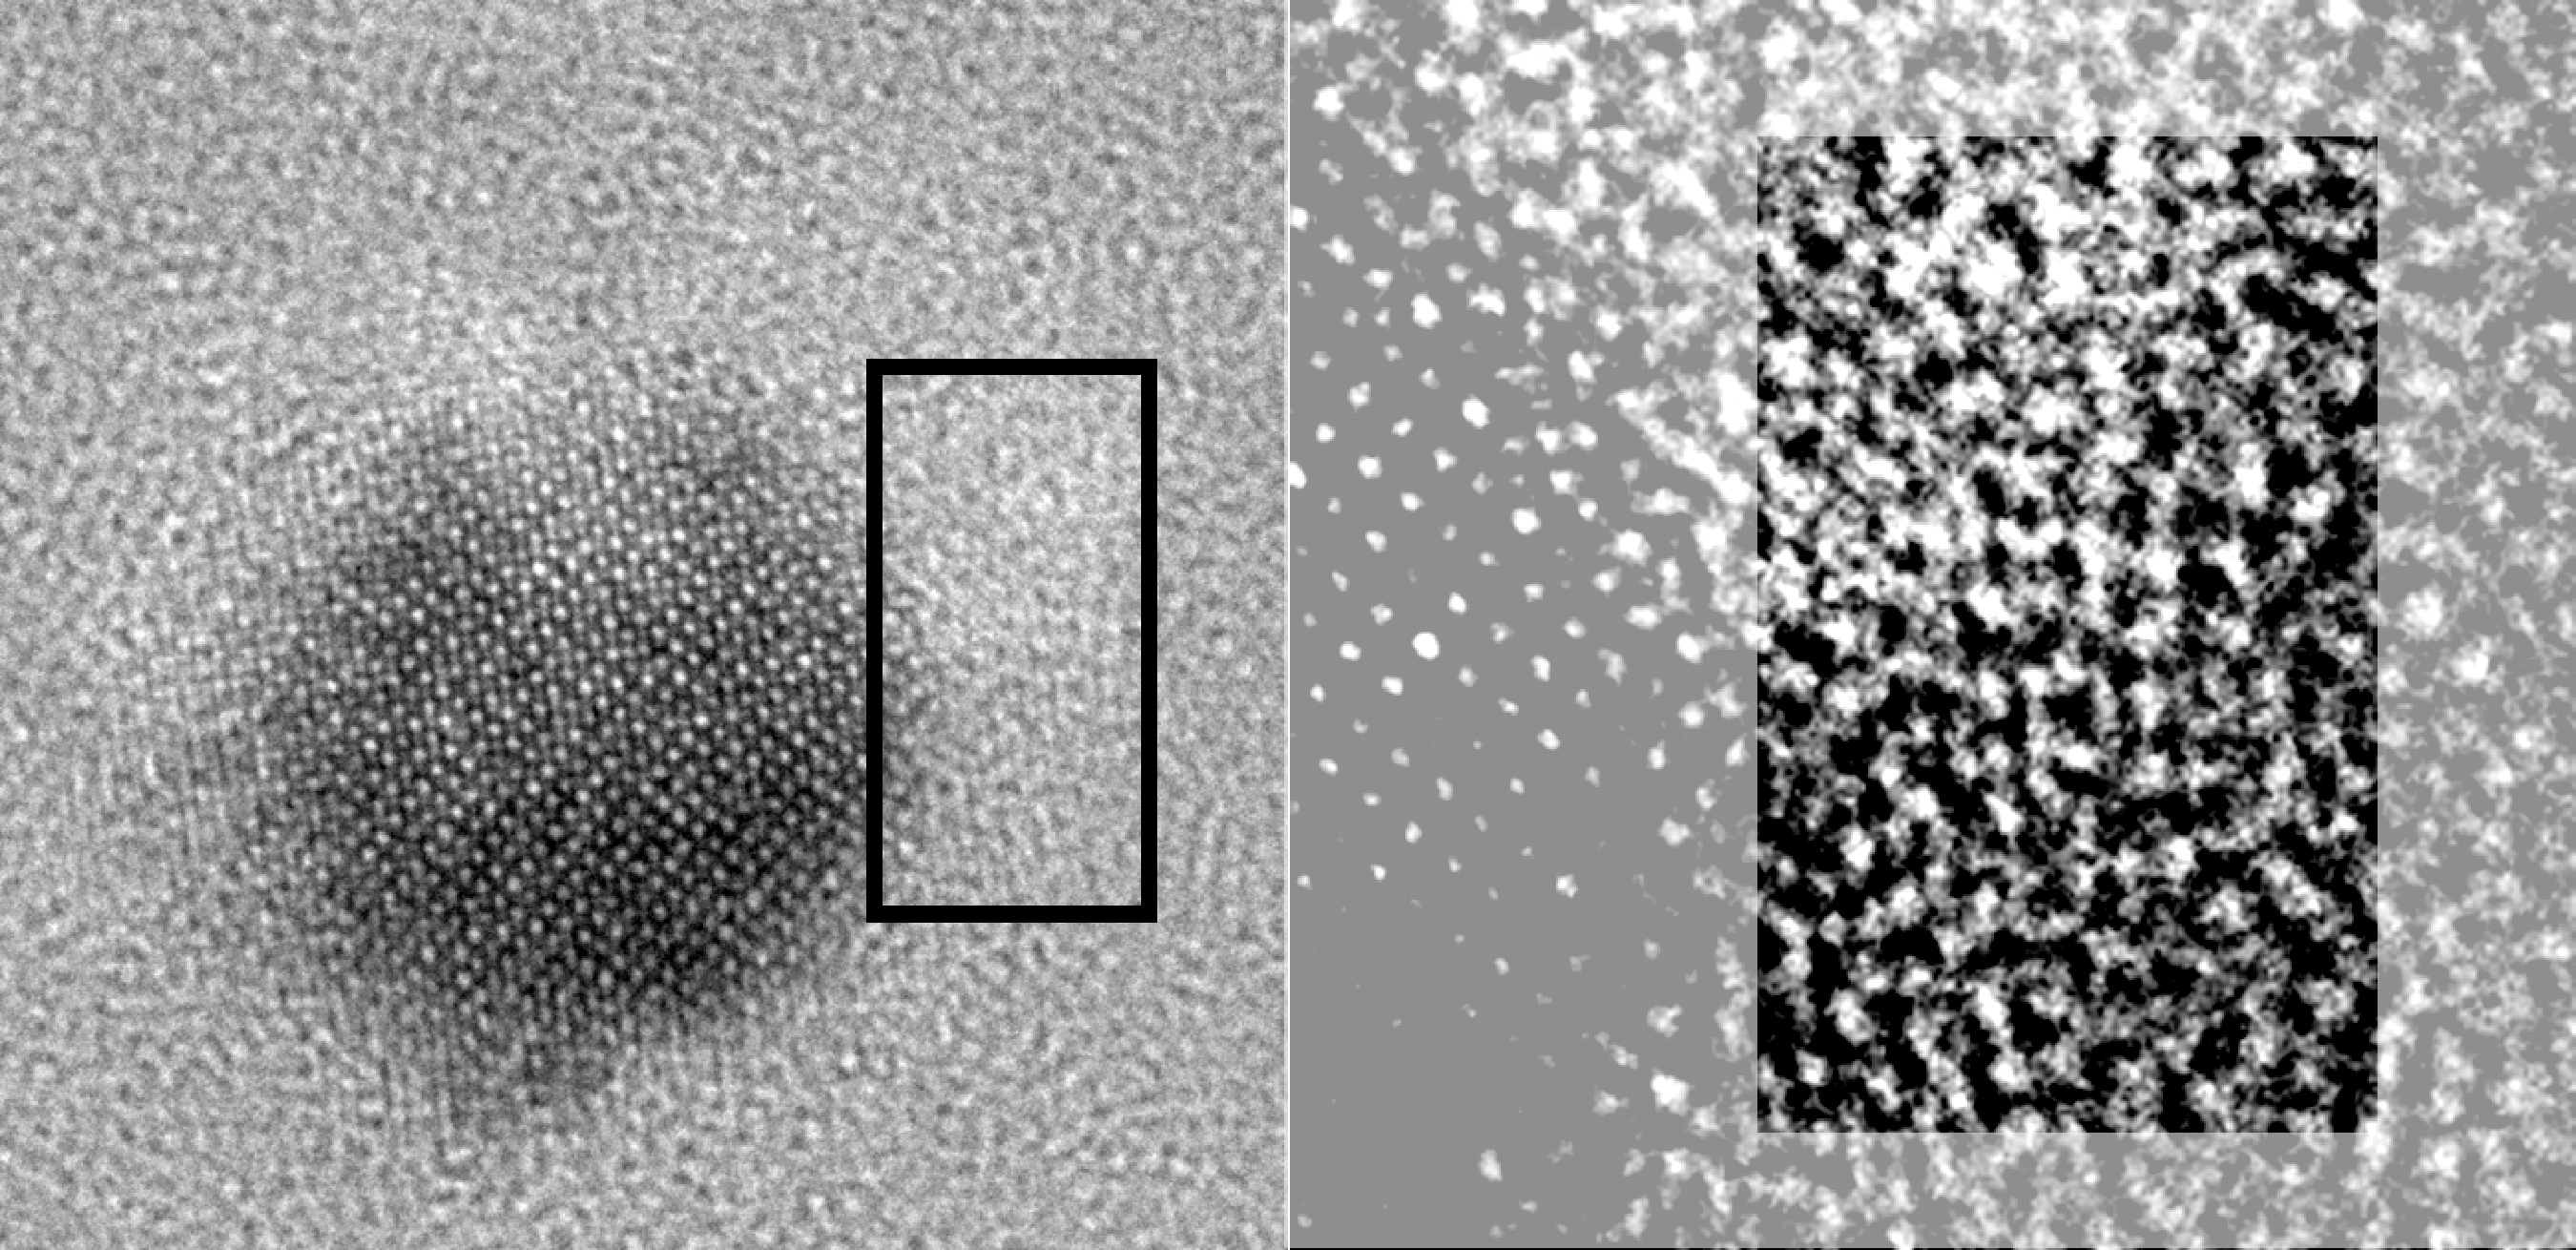
\includegraphics[width=0.8\textwidth]{figures/threading2.pdf}
    \caption{Image showing HRTEM of an Fe\textsubscript{2}O\textsubscript{3} nanoparticle with image intensity from higher $k$ vector, in focus outside boundary of nanoparticle highlighted(right)}
    \label{fig:fe2o3}
\end{figure}
Hence at the exact focus when circle of confusion is least, lattice with higher $k$ values are spread around and form an image away from where it should be located if image intensities were spatially correct (\textit{e.g.} see Figure~\ref{fig:fe2o3}).
This spreading of intensities is called Threading.

This also shows that for a field emission microscope, where beam coherence, and hence consequently, information limit, is large, information for higher $k$ vector or lower lattice spacings is still present in the image.


\begin{wrapfigure}{L}{0.5\textwidth}
    \centering
        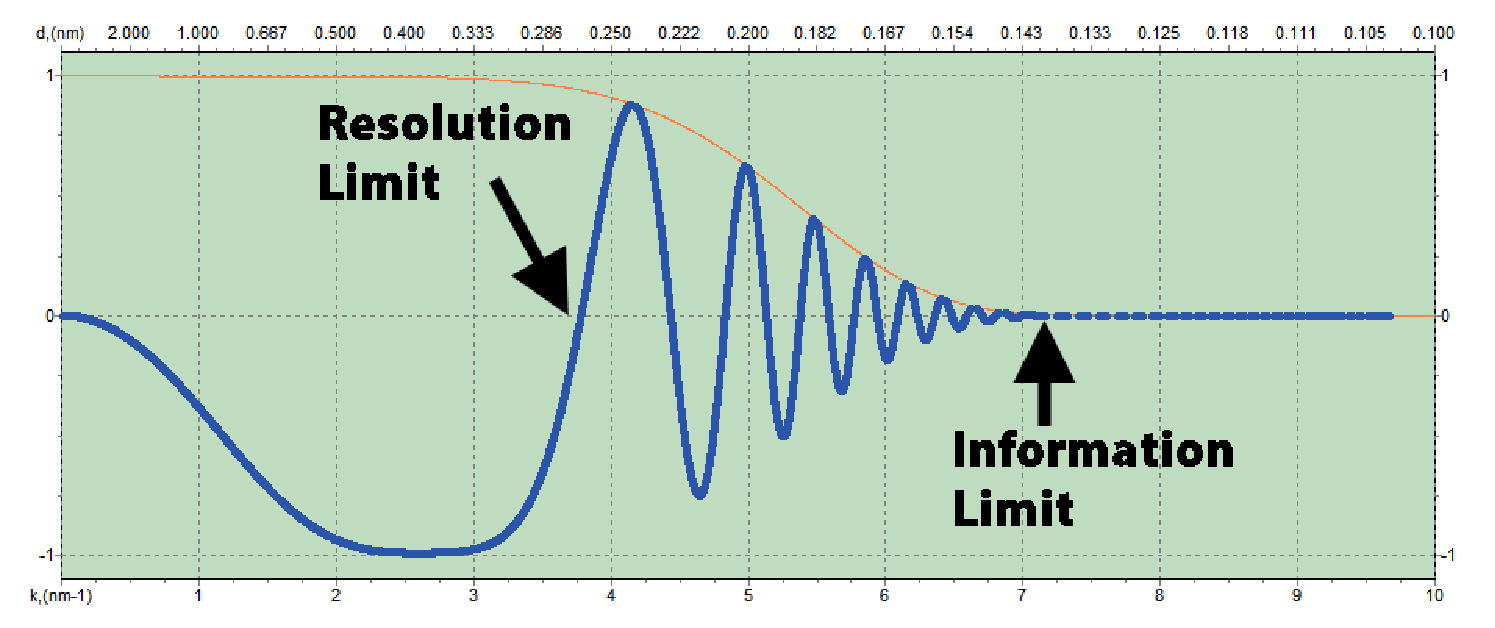
\includegraphics[width=0.5\textwidth]{figures/scherzer.pdf}
        \caption{Image showing CTF of a TEM at Scherzer defocus, with arrows to indicate resolution and information limit}
        \label{fig:ctfsherz}
\end{wrapfigure}


\subsection{Resolution Limit and Defocus} 

Resolution limit of any electron microscope is defined as the point where CTF crosses the zero for the first time (See Figure~\ref{fig:ctfsherz}).
Information Limit on the other hand is the limit of all the information about the sample present in the image.
By information present it means all the spatial frequencies that are imaged, irrespective of their contrast or location (threading).
Hence by above definition, Resolution limit is usually limited by defocus and more importantly spherical aberration while Information limit is decided by the beam decoherence and hence by chromatic aberration and environmental stability.

Point resolution of electron microscope, which as be described as the limit till which electron microscope can reproduce sample information linearly is defined as the point where CTF crosses zero when objective lens is focused at `Scherzer Defocus'.
Otto Scherzer defined `Scherzer' defocus as the defocus value where maximum linear behavior is obtained.
He demonstrated that above condition is met when following equation holds true\cite{Scherzer1949}
\begin{equation}
    \Delta f_{Scherzer} = -\sqrt{\frac{4}{3}\lambda C_s}
    \label{eq:scherzerdefocus}
\end{equation}

If above is met then from equation~\ref{eq:ctf} it can be shown that point resolution of electron microscope can be defined as:
\begin{equation}
    \rho_r \approx 0.66 (C_s \lambda^3)^{\frac{1}{4}} 
    \label{eq:pointresol}
\end{equation}

\begin{figure}[b]
    \centering
        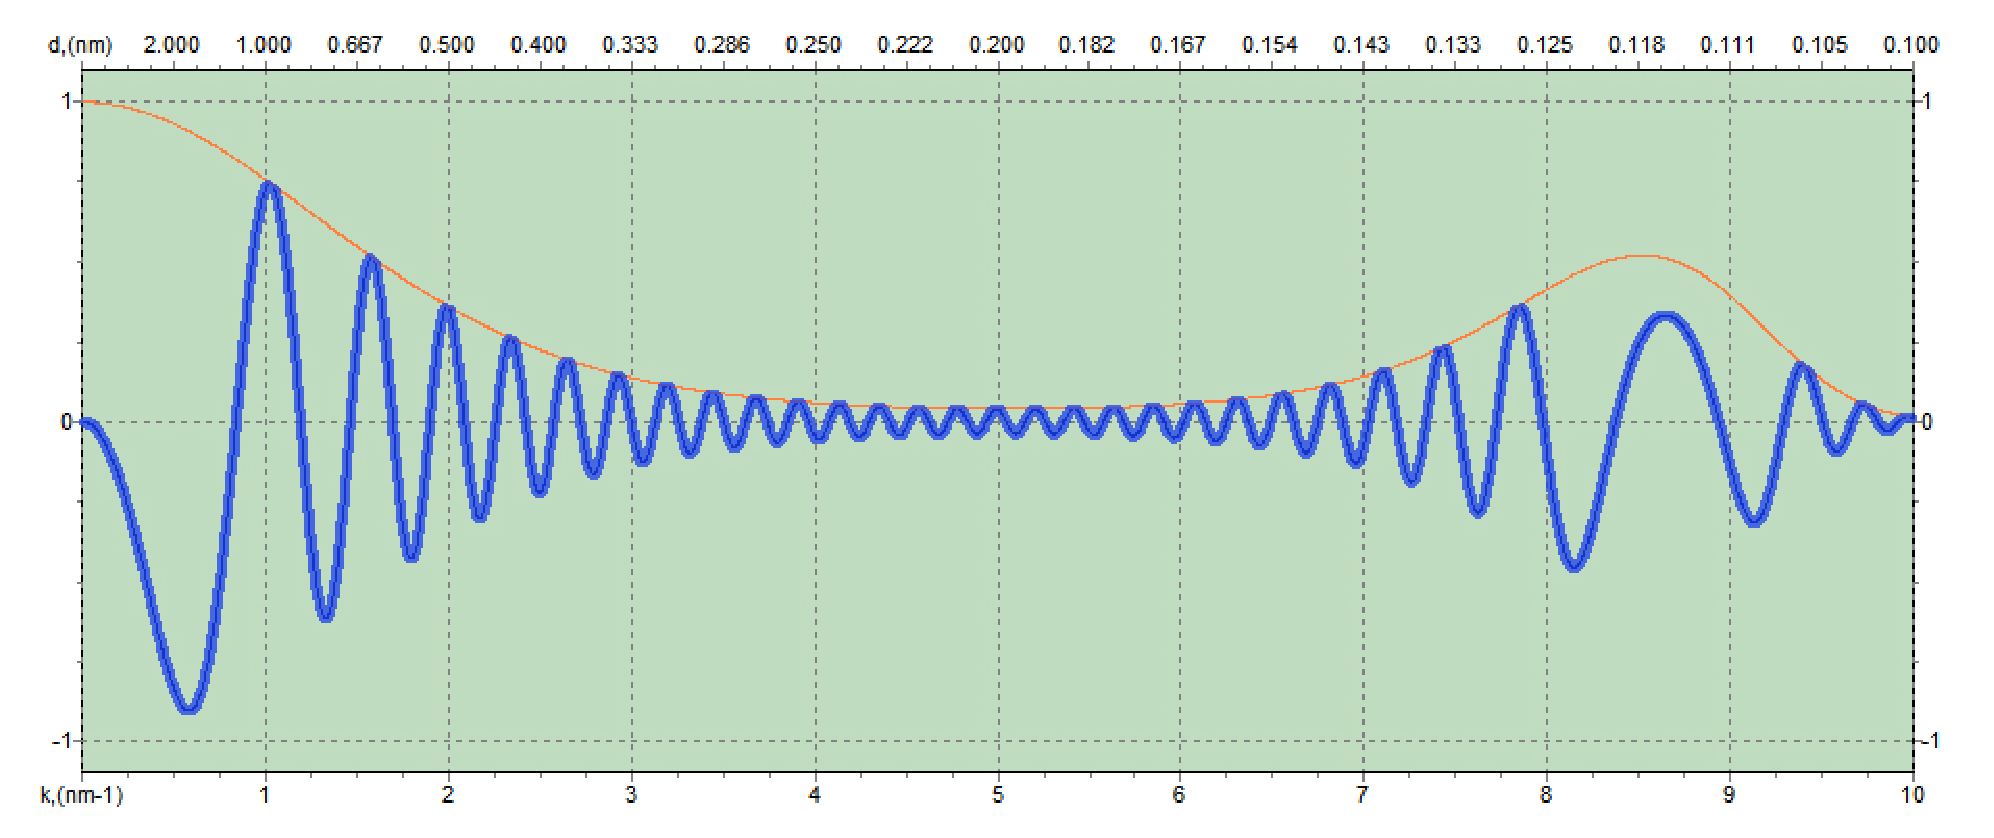
\includegraphics[width=0.5\textwidth]{figures/lichte.pdf}
        \caption{Image showing CTF of a TEM at Lichte defocus}
        \label{fig:ctflichte}
\end{figure}


All of the HRTEM work is preferably done at Scherzer defocus, as it produces most simple to interpret images.
Sometimes `Extended Scherzer', defined as $1.2 \Delta f_{Scherzer}$, is used for HRTEM, where slight linearity is sacrificed to gain more resolution by pushing the resolution limit.
Another important imaging condition is call Lichte defocus.
Described by Hannes Lichte, it is best suitable for holographic reconstructions, as it tried to maximize the information gathered by pushing the decoherence envelope function.\cite{Lichte1991}
Because of large fluctuation in contrast as such (Figure~\ref{fig:ctflichte}), Lichte defocus has little use outside electron holography.
\begin{figure}[t]
    \centering
    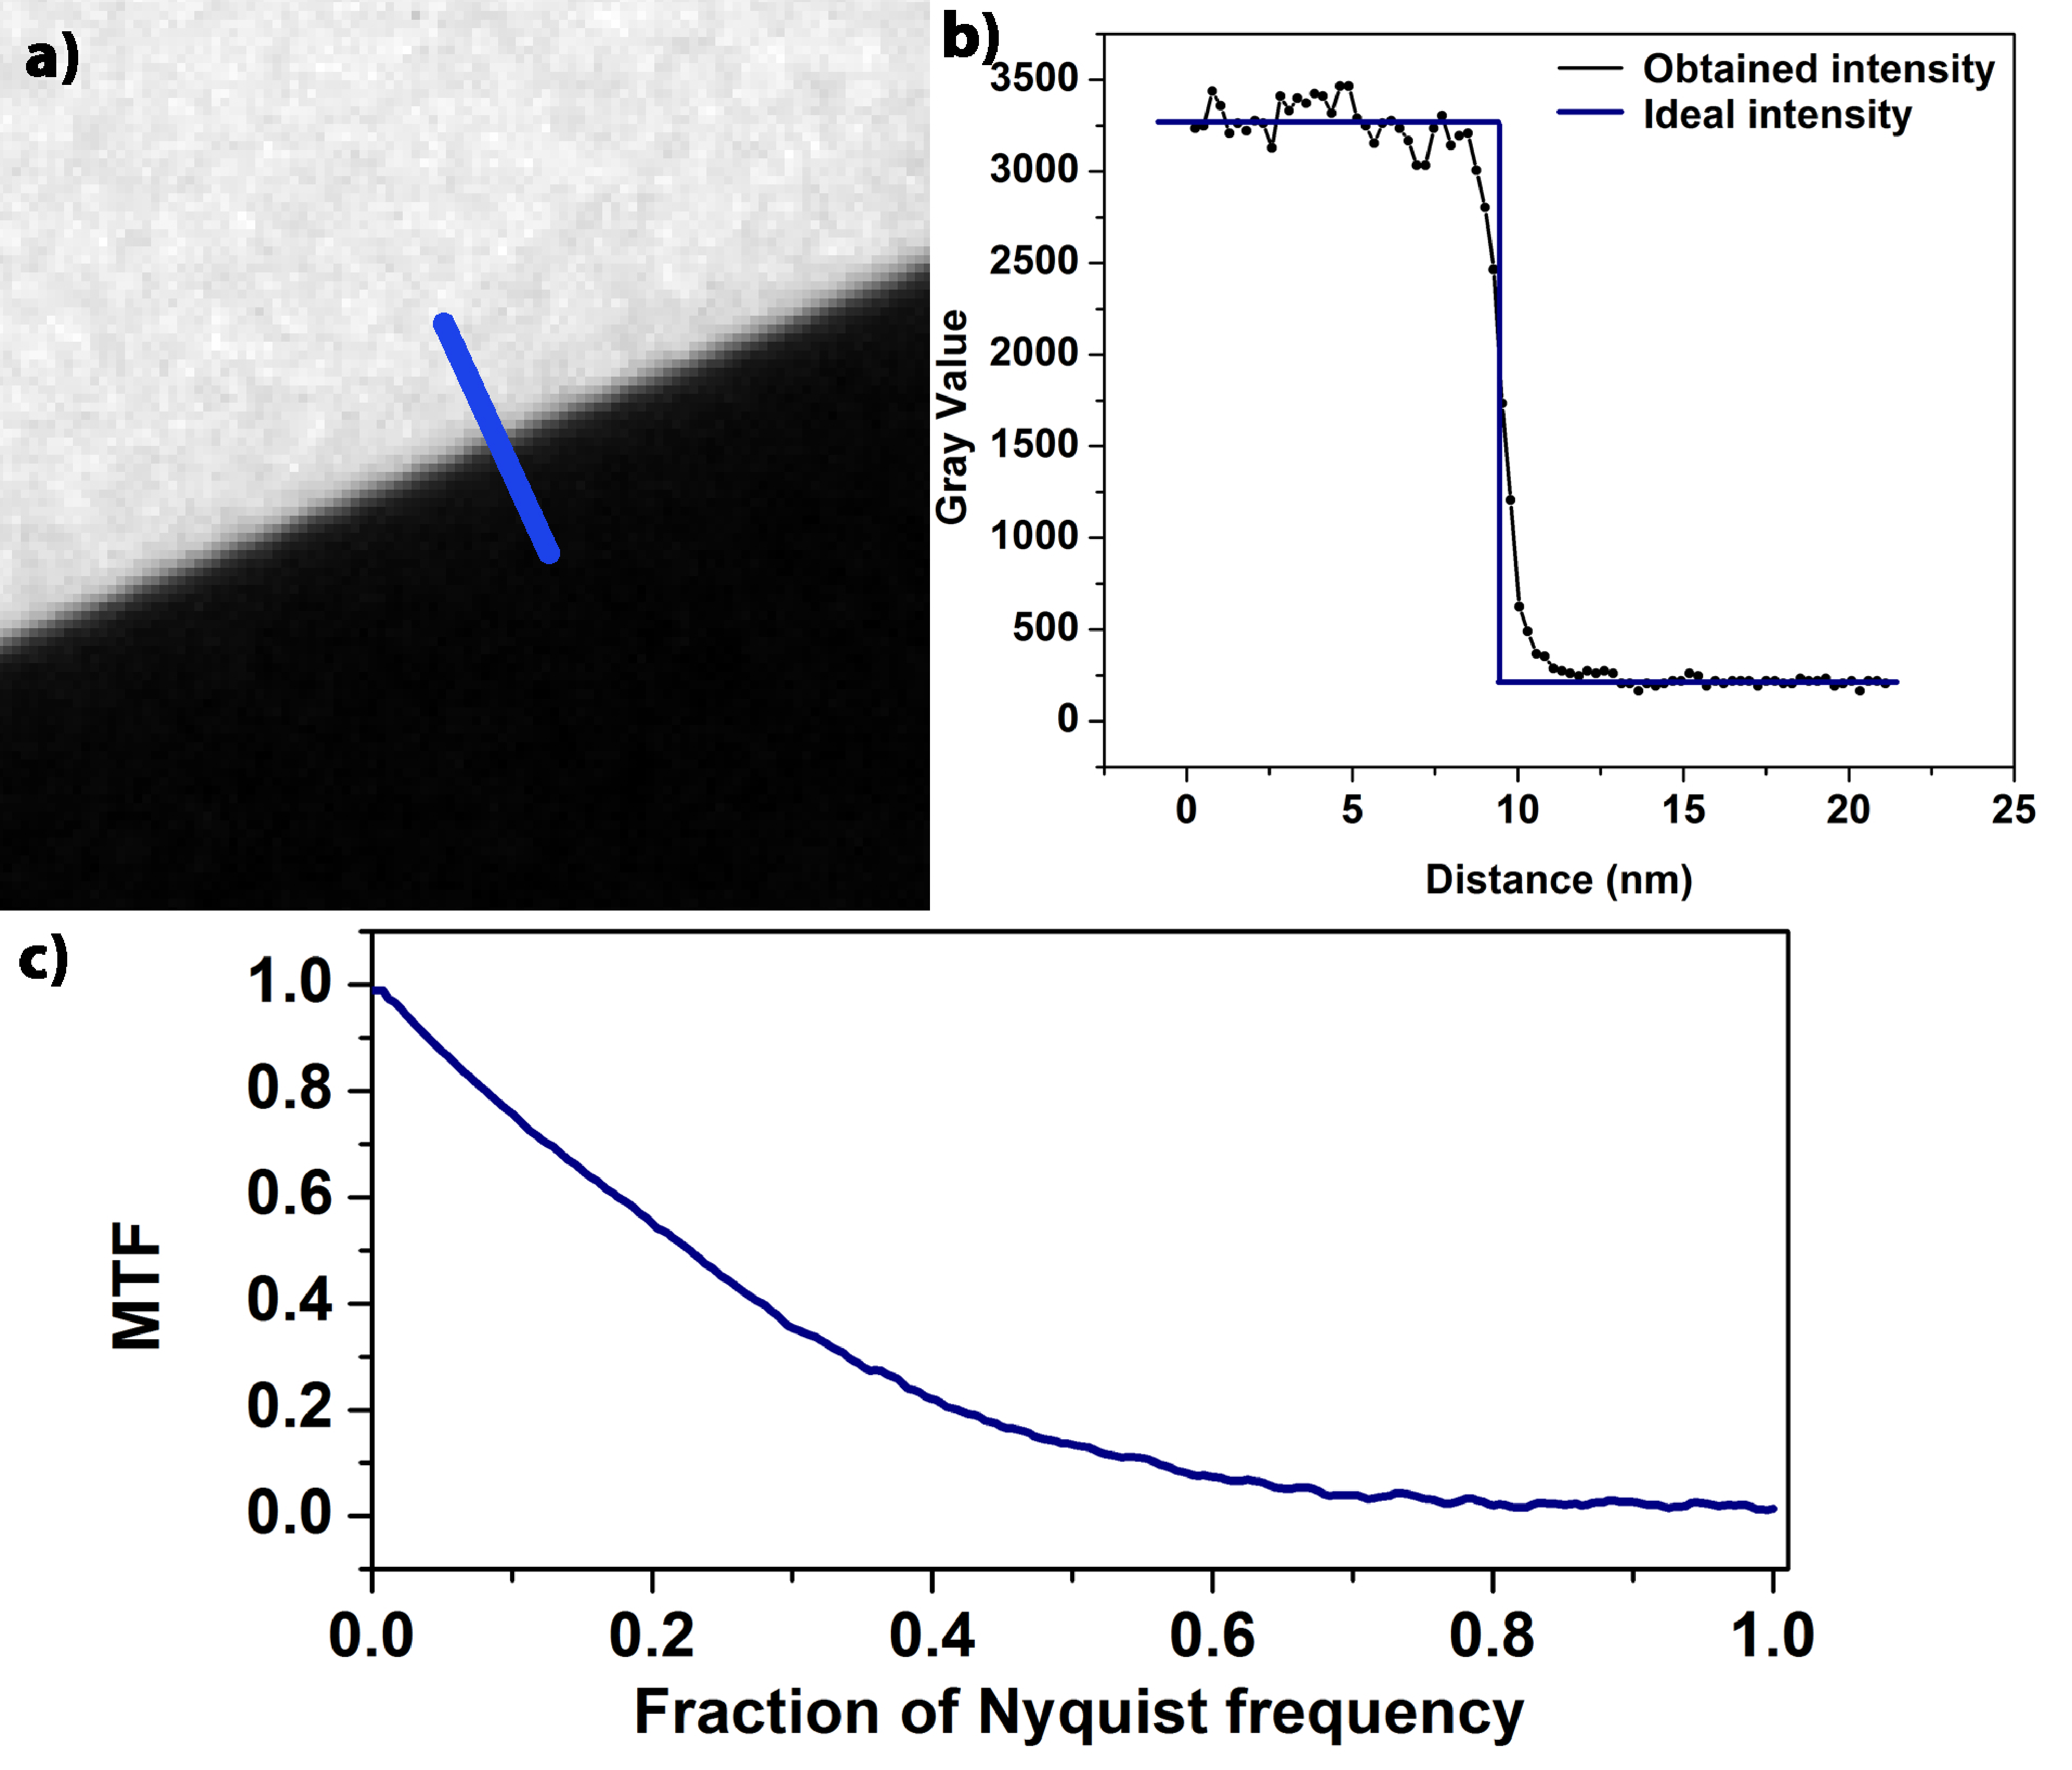
\includegraphics[width=0.9\textwidth]{figures/MTFtheory.pdf}
    \caption{a) A zoomed out image of a shadow of beam blocker, showing diffused edges, b) graphs showing `perfect' edge step function and actual intensity levels along the blue line shown in image (a), and c) MTF of a Olympus-SIS KeenView G2 CCD camera fitted under a JEOL JEM 2100F TEM used in this document (Generated by MTFestimate program, donated generously by Dr. Wouter Van den Broek \cite{VandenBroek2012})}
    \label{fig:mtfall}
\end{figure}

Lichte defocus is given by:
\begin{equation}
    \Delta f_{Lichte} = -\frac{3}{4} C_s (q_{max} \lambda)^2
\end{equation}
Here $q_{max}$ is the maximum spatial frequency till which information is available.
It is limited by objective aperture or information limit.

\subsection{Modulus Transfer Function (MTF)}
Till now we discussed only about the electron microscope and its physical limitations.
Final step in any image acquisition is it image formation on the camera.
For CCD cameras, which are most used ones today, a unique problem arises, that is of transfer of contrast from a periodic image.

In ideal case any camera should be able to record exact intensities from the sample, \textit{i.e.} if we place any opaque object in its path then opaque areas shall be dark or intensity shall be zero, while transparent areas shall be completely bright.
However due to construction of CCD and due to quantization of image in terms of pixels, contrast transfer as such is not perfect and there is a transition zone in which contrast will go from zero to desired value as a sinusoidal function (Figure~\ref{fig:mtfall}a and b).

If we now consider any periodic lattice, which is being imaged, we can see that how the contrast levels of that lattice spacing will depend on the camera (\textit{e.g.} Figure~\ref{fig:mtfexample}).

\begin{figure}[b]
    \centering
    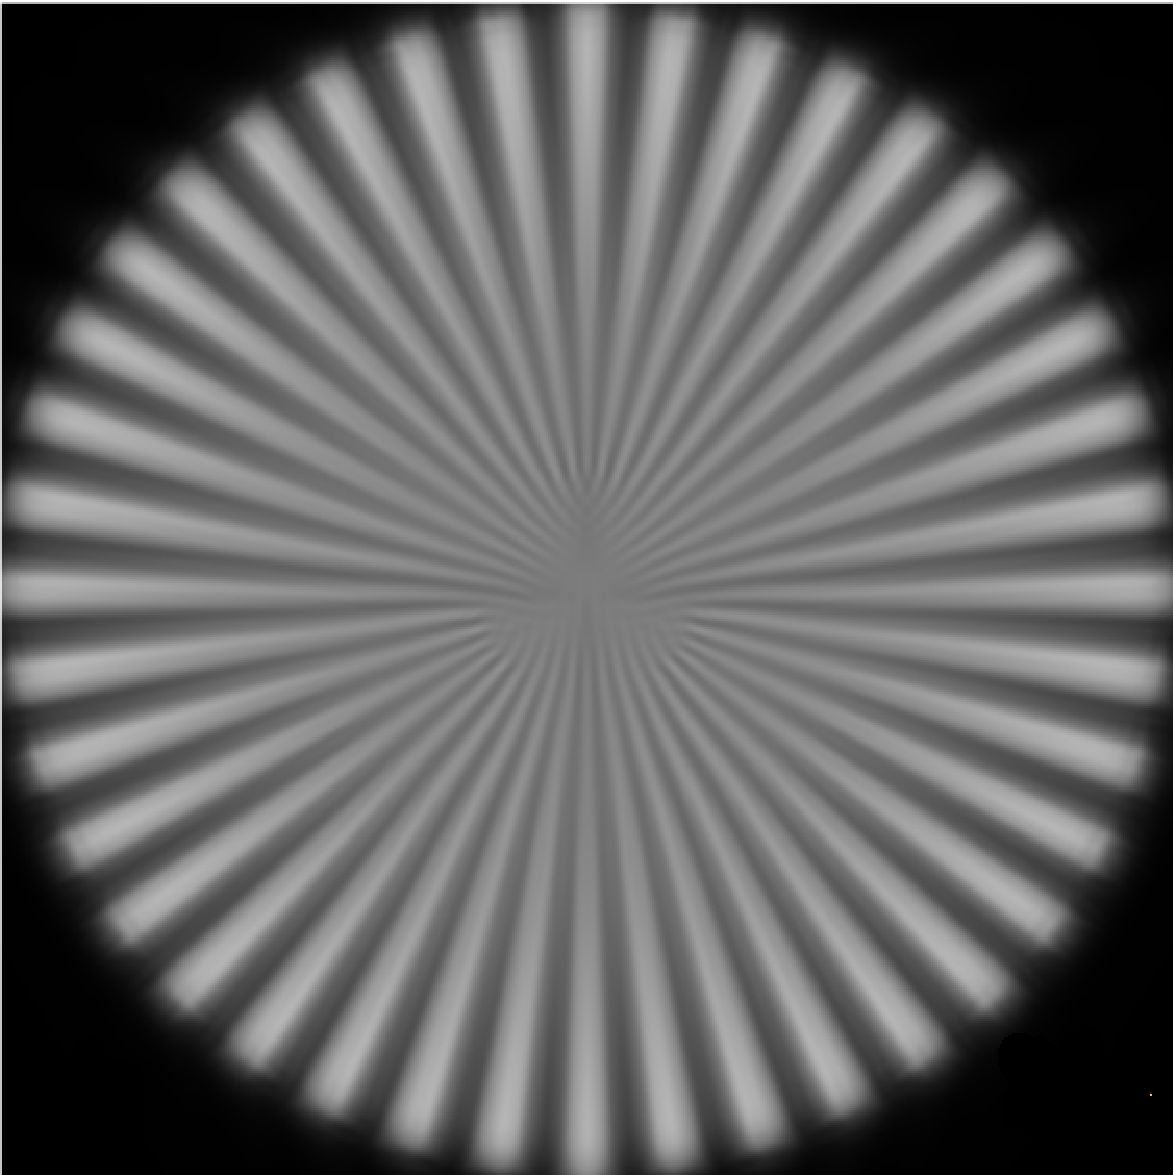
\includegraphics[width=0.30\textwidth]{figures/mtfeg.pdf}
    \caption{An image showing change in contrast of an image recorded on digital camera, as we go from lower spatial frequency to higher spatial frequencies [image credit:Tom.vettenburg, via Wikimedia Commons]}
    \label{fig:mtfexample}
\end{figure}

This relation between the difference in contrast between dark and light fringes for a periodic spacing being imaged is called Modulus Transfer Function or MTF of the camera.
Ideally it should be 1 as all frequencies shall be reproduced with actual contrast, however for an actual camera it looks like as shown in Figure~\ref{fig:mtfall}c.

For further details please consult \cite{VandenBroek2012,Koeck2000}
    %!TEX root=./main.tex
\section{Theory and Algorithms}
As explained in previous section, idea behind deconvolution of images, or any signal for that matter, is simple: divide fourier transform of the point spread function from fourier transform of image to get pure image object \textit{i.e.} from equation~\ref{eq:fourierconv}:
\begin{equation}
    \psi_t(x)= IFFT\{\Psi_i(\boldsymbol{k}) / H_o(\boldsymbol{k})\}
\end{equation}
where:
\begin{description}
    \item[IFFT] is inverse fourier transform operation
\end{description}
However there is one problem: transfer function $H_o(\boldsymbol{k})$ is oscillatory in nature and crosses zero several times (Figure~\ref{fig:ctffigure}).
Hence it results in division by zero error or amplification of noise.
Essentially whenever transfer function nears zero, that portion shall be avoided. 
To facilitate this one of the earliest approach was \textit{Parabola Approximation Method}\cite{OpdeBeeck1996}, where variation in defocus makes several `pass bands' which creates a linear region of contrast transfer in CTF.
As per previous reference, as linear contribution to HRTEM image comes from direct beam and diffracted beam, it can be shown that intensity of image in fourier space $I(\Psi(\boldsymbol{g}),\zeta)$ is proportional to:
\begin{equation}
    \frac{exp(-[\{\zeta - 0.5\lambda(g^2 + 2\boldsymbol{g.p})\}/\pi\alpha g])}{\pi\alpha g}exp(\iota 2 \pi C_s \lambda ^2\{g^2 + 3(p^2 + \boldsymbol{g.p})\}\{\zeta - 0.5 \lambda (g^2 + 2\boldsymbol{g.p})\})
    \label{eq:debeeckfourierI}
\end{equation}
where $\zeta$ represents inverse defocus in fourier space.
For parallel beams (\textit{i.e.} $\alpha = 0$), the first term in equation~\ref{eq:debeeckfourierI} reduces to Dirac delta function of form $\delta (\zeta - 0.5\lambda (g^2 + 2\boldsymbol{g.p}))$. 
ignoring the non-linear part this reduces to:
\begin{equation}
    \zeta = \pm 0.5\lambda g^2
\end{equation}
It is equivalent to propagation along Ewald sphere, where Ewald sphere is parabolic due to Fresnel approximation used in deriving the image intensity equation (see `Parxial approximation' of Helmholtz equation\cite{Hecht2002}). 
\begin{figure}[htp]
    \centering
    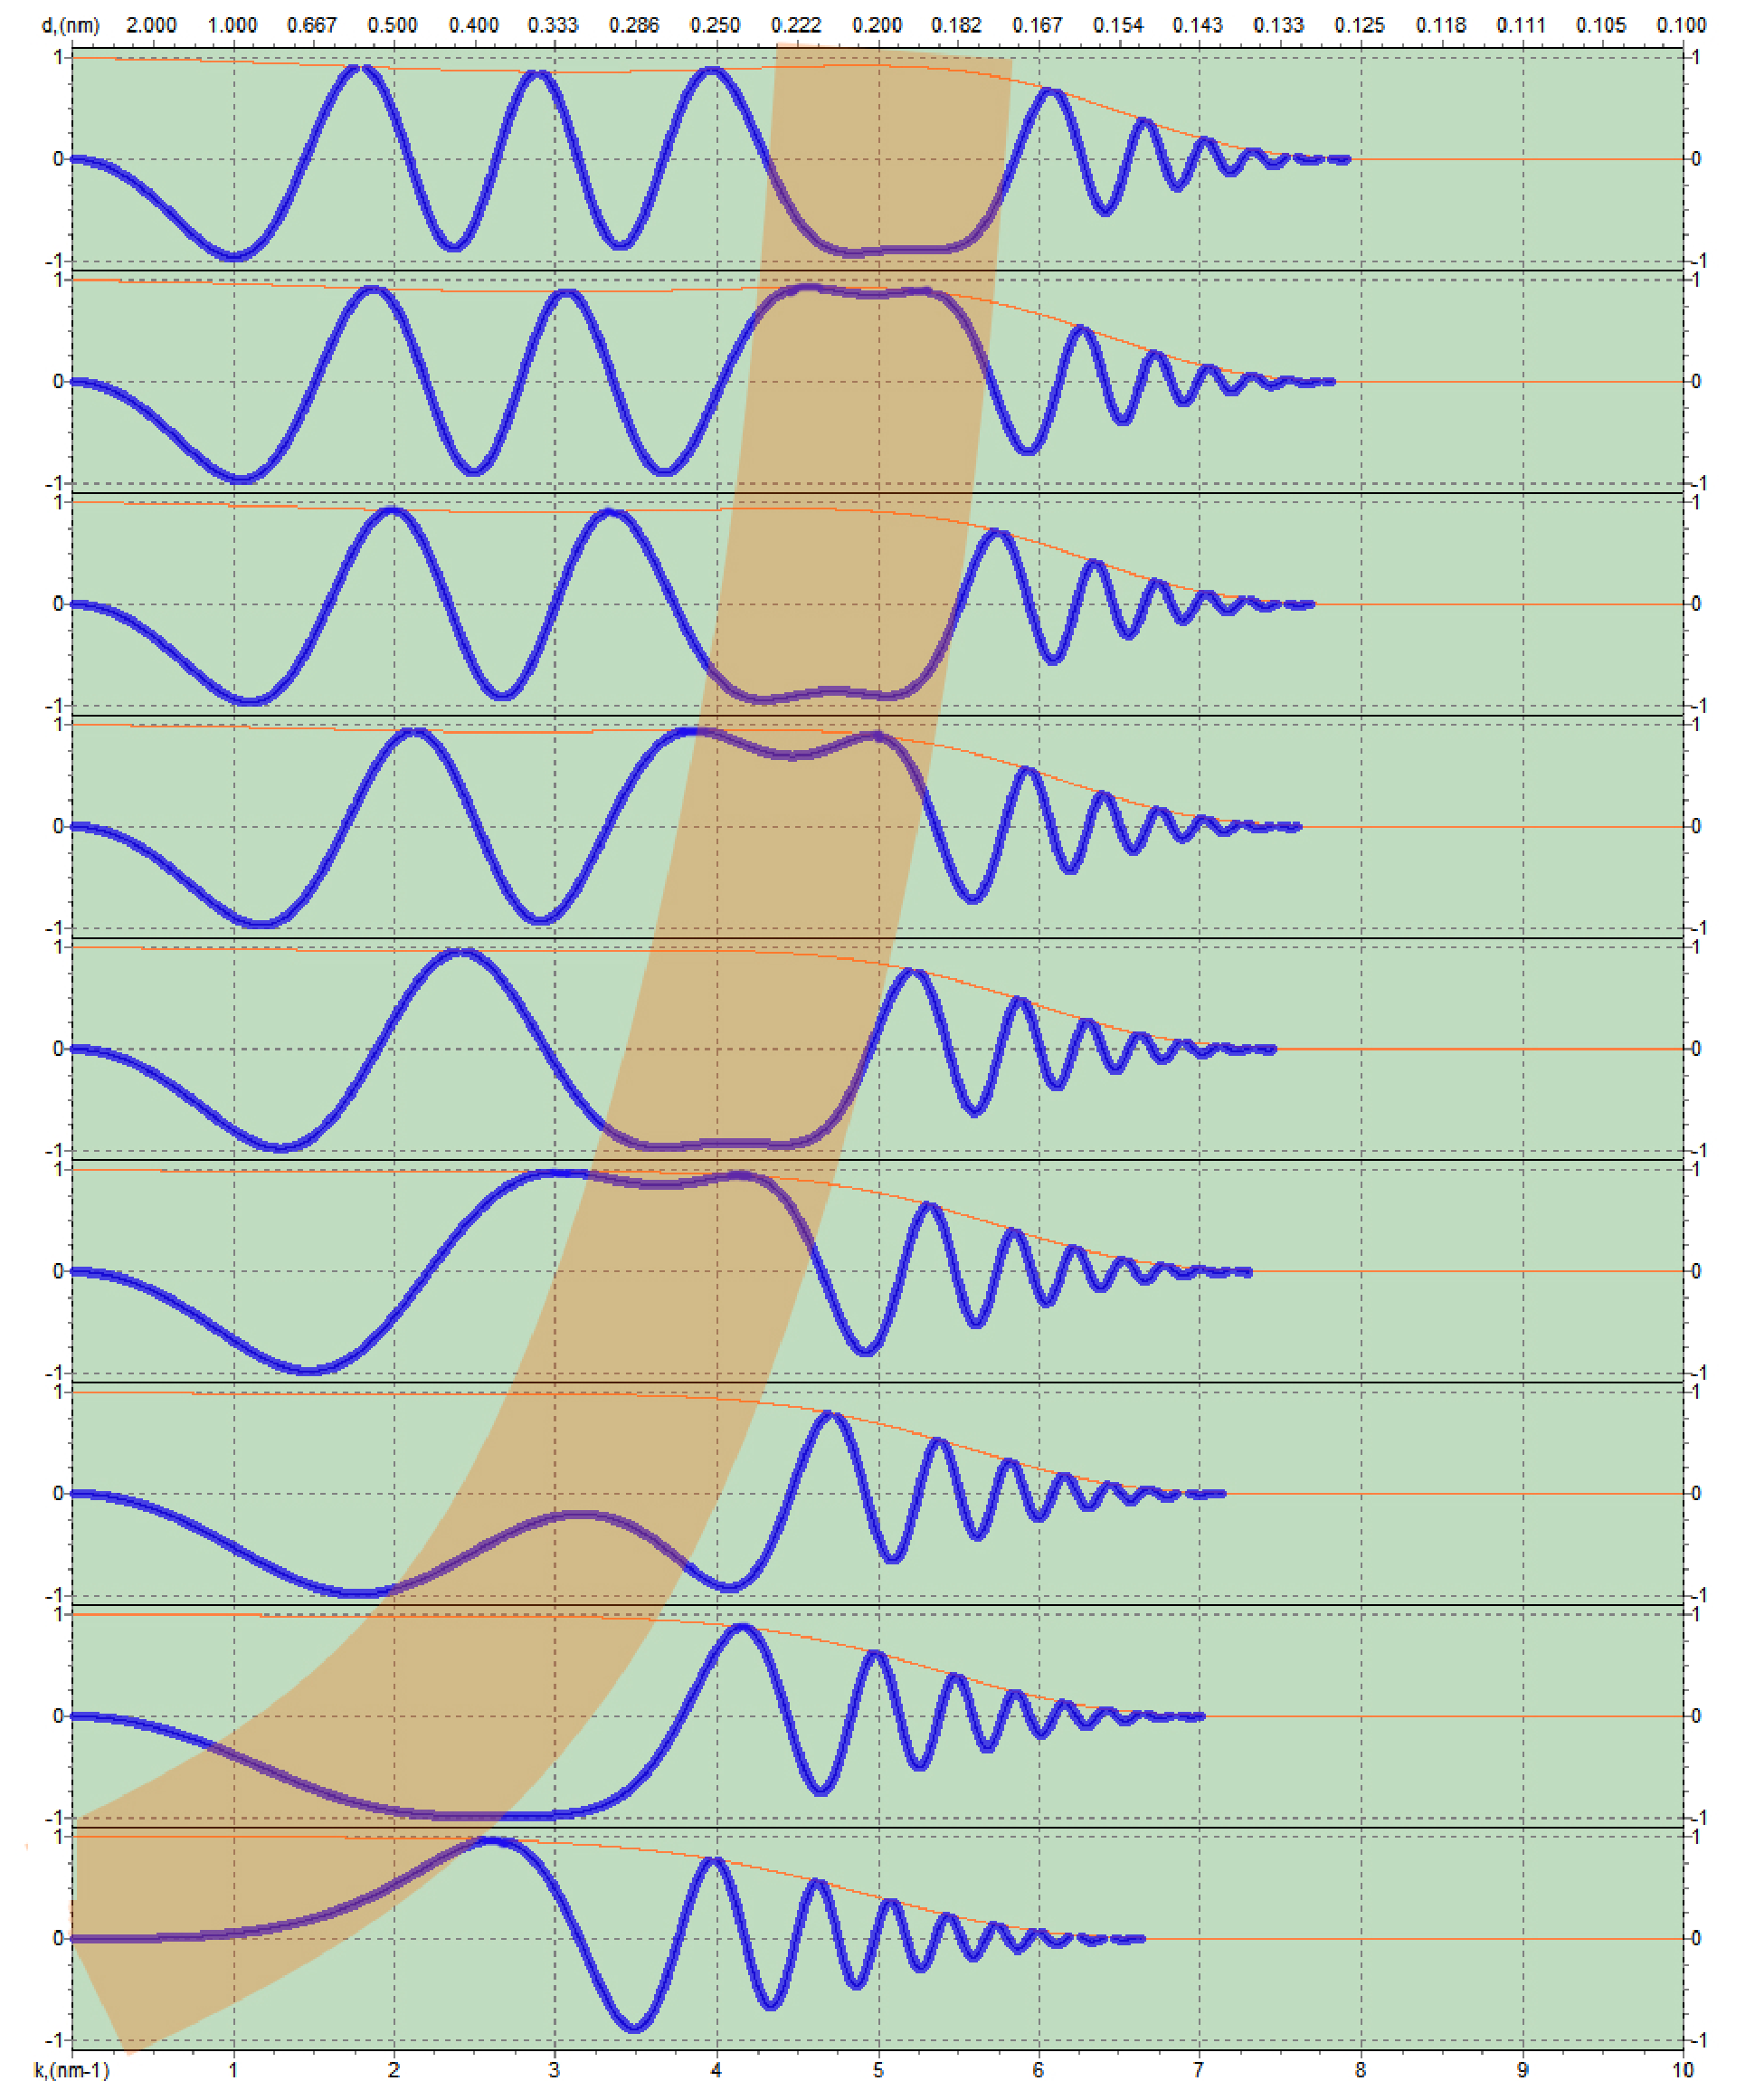
\includegraphics[width=\textwidth]{figures/ctfparabola.pdf}
    \caption{CTF showing propagation of linear pass bands with increase in defocus}
    \label{fig:ctfparabola}
\end{figure}


Hence all such pass bands (where $\boldsymbol{p}=0$ and $\boldsymbol{p}+\boldsymbol{g}=0$) lie on a paraboloid of a 3D Fourier transform of image stack, where 3rd dimension is defocus value.
Propagation of such pass bands with defocus in CTF is shown in Figure~\ref{fig:ctfparabola}. 
So basic principle is to get unaberrated linear contributions from various pass bands and stitch them together.


% \begin{wrapfigure}{}{\textwidth}
\begin{figure}[!ht]
    \centering
    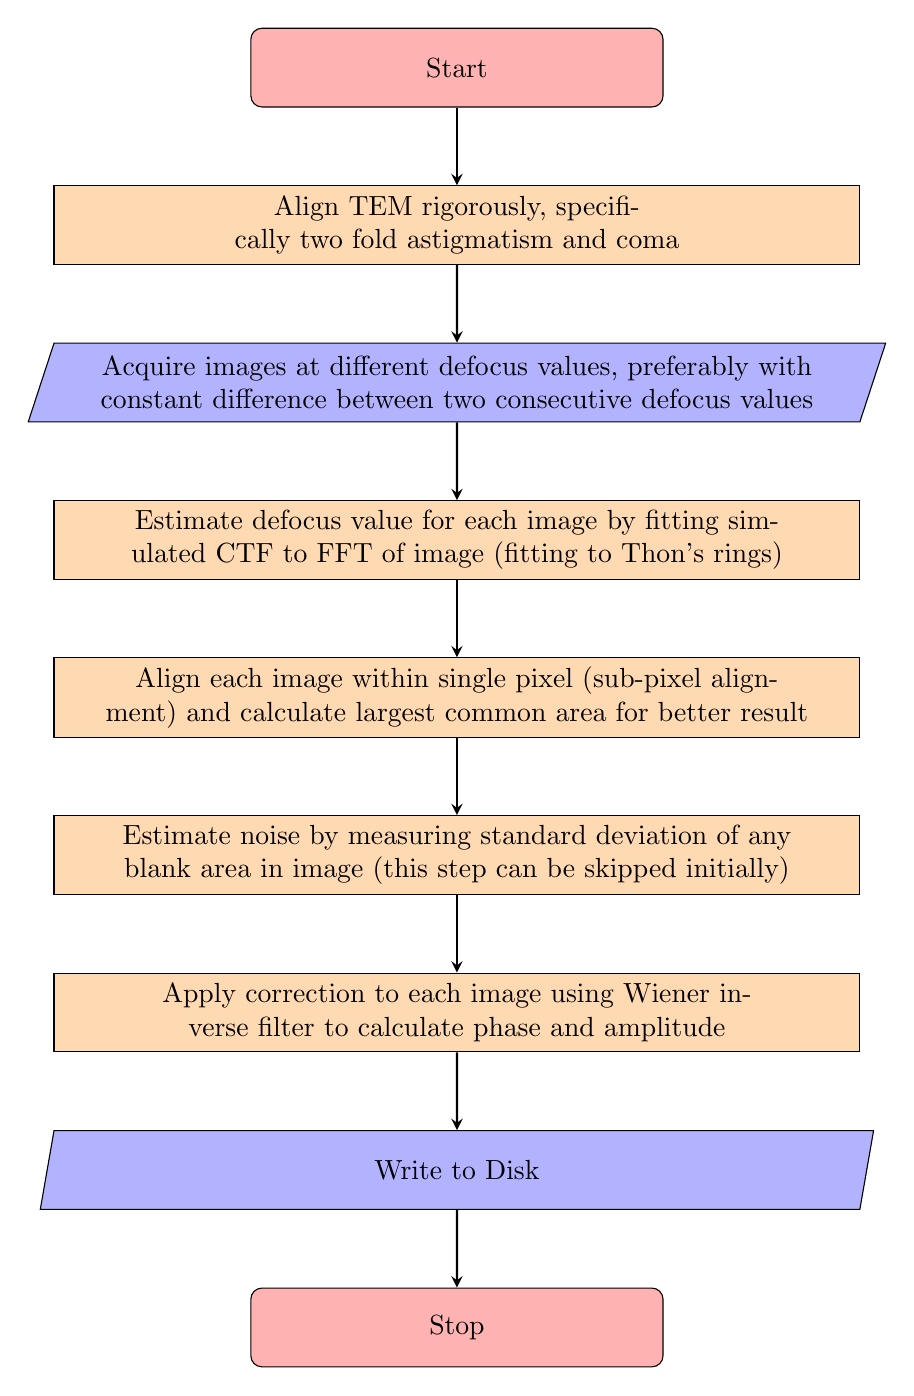
\begin{tikzpicture}[node distance=2cm]
        \node(start) [startstop] {Start};
        \node(proc1) [process,below of = start] {Align TEM rigorously, specifically two fold astigmatism and coma};
        \node(in1) [io,below of = proc1] {Acquire images at different defocus values, preferably with constant difference between two consecutive defocus values};
        \node(proc2) [process,below of = in1] {Estimate defocus value for each image by fitting simulated CTF to FFT of image (fitting to Thon's rings)};
        \node(proc3) [process,below of = proc2] {Align each image within single pixel (sub-pixel alignment) and calculate largest common area for better result};
        \node(proc4) [process,below of = proc3] {Estimate noise by measuring standard deviation of any blank area in image (this step can be skipped initially)};
        \node(proc5) [process,below of = proc4] {Apply correction to each image using Wiener inverse filter to calculate phase and amplitude};
        \node(out1) [io,below of = proc5] {Write to Disk};
        \node(stop) [startstop, below of = out1] {Stop};
        % \node(dec1) [decision,below of = proc1,yshift=-0.5cm] {yes we can?};
        % \node(proc2) [process, right of = dec1,xshift=2cm] {here we go again};
        % \node(proc3) [process, below of = dec1,yshift=-0.5cm] {last chance};
        % \node(out1) [io, below of = proc3] {here it comes};
        % \node(end) [startstop, below of = out1] {Stop};
        \draw [arrow] (start)--(proc1);
        \draw [arrow] (proc1)--(in1);
        \draw [arrow] (in1)--(proc2);
        % \draw [arrow] (dec1)--node[anchor=west] {yes} (proc3);
        % \draw [arrow] (proc2)|-node[anchor=west] {no} (proc1);
        \draw [arrow] (proc2)--(proc3);
        \draw [arrow] (proc3)--(proc4);
        \draw [arrow] (proc4)--(proc5);
        \draw [arrow] (proc5)--(out1);
        \draw [arrow] (out1)--(stop);
    \end{tikzpicture}
    \caption{Basic schematic for Exit wave reconstruction}
    \label{fig:basic1}
\end{figure}
% \end{wrapfigure}


It can be demonstrated that above condition can be reduced to a special case called \textit{Wiener Inverse Filter}, before dwelling into detail, given here (Figure~\ref{fig:basic1}) is a simple algorithm for exit wave reconstruction.

\textbf{1. Alignment:}
Other than the usual TEM alignment, following things need to be paid special attention to: Condenser aperture, Objective astigmatism (2-fold), Coma.
Usually 2nd condenser aperture is a good compromise between intensity and coherence in HRTEM.
Two fold astigmatism can be removed from image by observing live FFT of amorphous background near region of interest on screen and compensating it with Objective stigmator till it is completely symmetric in both overfocus and underfocus condition.
Usually it can be corrected by measuring defocus in perpendicular directions and  numerically compensating it in Wave Aberration function\cite{meyer_symmetric}, but it has not been implemented yet in presented piece of code. 

It was found that coma correction yield better quality results than voltage centered images.
This can probably be explained by the fact that at high magnification, area of viewing is small hence small tilt in beam might not degrade image quality as much as the coma aberration.
Coma was corrected by rocking beam in x and y direction (under \textit{Maintenance \textgreater Alignment \textgreater Tilt X/Y}) while correcting tilt using \textit{bright tilt} in same direction, till FFT was same on both extremes of tilt.
Amplitude and frequency of rocking, and frame rate under CCD camera can be adjusted to aid if necessary. 

\textbf{2. Image Acquisition:}
Equation~\ref{eq:debeeckfourierI} was subjected to approximation that beam is parallel, \textit{i.e.} convergence angle is very low.
This can be ensured as following in JEOL microscopes by using $\alpha$1 mode (consult user manual on how to align it for the same).

Image drift shall be minimum while taking any images, it will not only give larger area to work upon (larger image area results in better less noisy FFT) but also drift results in streaking in images which looks like 2-fold astigmatism.
One of the simpler way to achieve above is to take a small video consisting for 20-30 frames and pick the frame that gives best results (a crude tool vid2img is provided for extracting frames from a video recorded from iTEM software).
Drift can be minimized by reducing exposure time as well, to compensate for decrease in intensity CCD camera's pixcels can be binned.
However such binning can be done later on numerically as well.

Once above is taken care of and image quality is of desired value, click 20-30 images at regular defocus, usually starting from slightly higher defocus value than Scherzer defocus as it is simpler to estimate defocus value from images in that region.
Pass bands can also be observed in live FFT which might aid in deciding the defocus interval.
Including small amount of amorphous carbon would be useful as well.

\textbf{3. Defocus estimation:}
If Spherical aberration coefficient of TEM is known accurately then defocus of any image can be determined by fitting minima of Thon's rings in FFT of images to the simulated CTF function.
For correct estimation of defocus value, CTF has to be simulated which requires accurate determination of spherical aberration coefficient.
For the microscope in use it was determined to be 0.95 mm, which is in close agreement with the quoted value, from the manufacturer, of 1.00 mm.
Spherical aberration coefficient was determined using tilt series cubic fit method.\cite{Koster1991} 
Defocus estimation by current method is slightly difficult if no amorphous carbon is present in image or if images are too close to exact defocus.
For defocus estimation \texttt{defocus\_esimation.m} GUI has been provided in current codes.

\begin{figure}
    \centering
    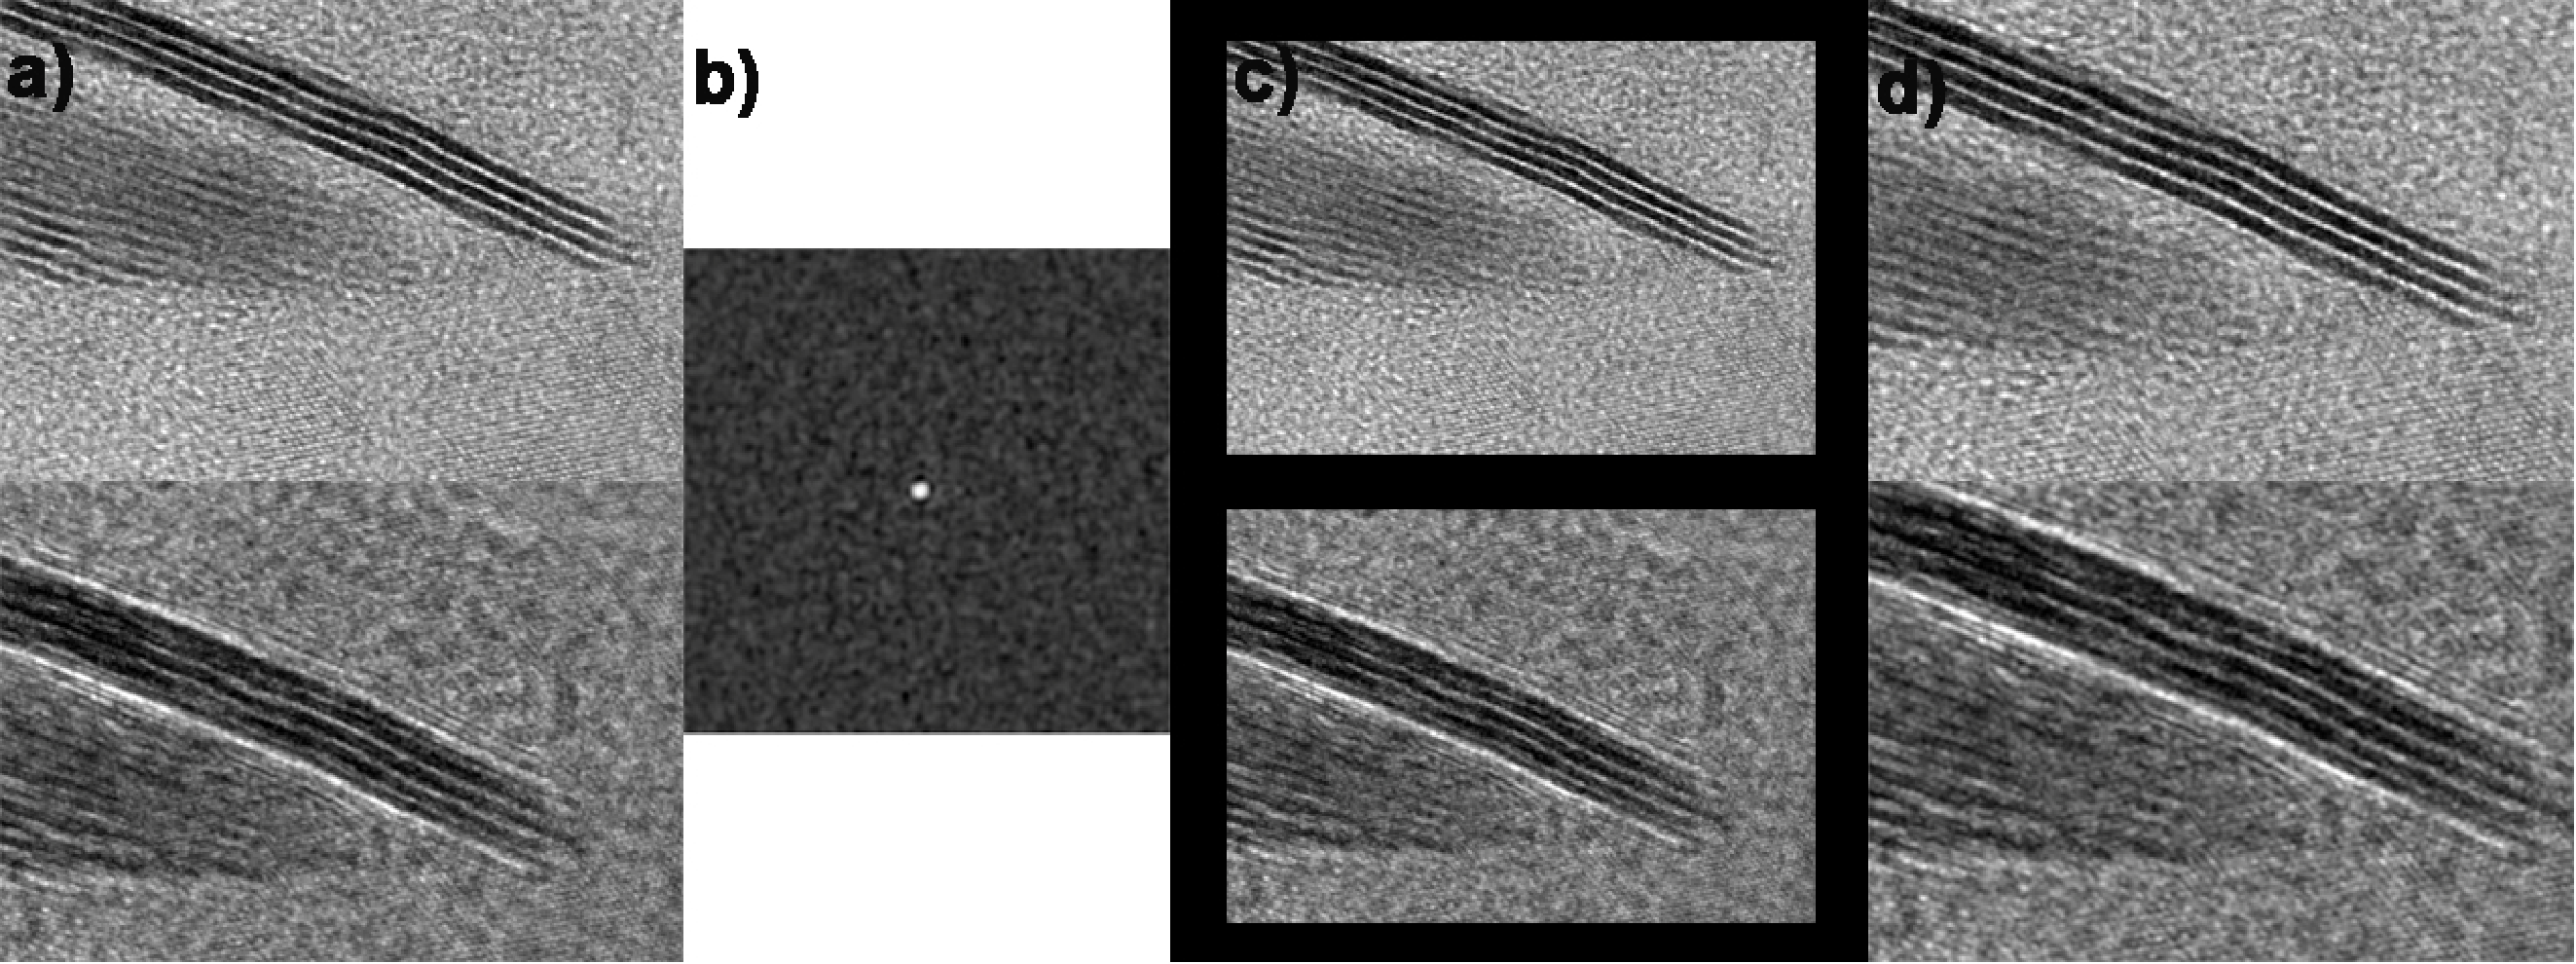
\includegraphics[width=\textwidth]{figures/LargestArea.pdf}
    \caption{Schematic representation of largest common image area selection and sub pixel alignment, a) initial images with large shift/drift, b) phase correlation peak between 2 images, c) padded and shifted images and d) common area of both images}
    \label{fig:subpixel}
\end{figure}

\textbf{4. Sub-pixel alignment:}
Sub-pixel alignment was divided into two parts: i) selection of largest common area in images, ii) sub-pixel alignment of the selected area.
To achieve this first phase correlation between all images were determined (\texttt{pcorr.m} file contains phase correlation code).
Following the determination of shift in each image, maximum shift was determined by summing all individual shifts (Figure~\ref{fig:subpixel}a and b).
To facilitate alignment of images, finally a blank padding was added to the images.
The width of padding was chosen to be slightly more than the total displacements among images.
All such shifted images were added in a single matrix, followed by binarization of the matrix, which then yields the mask which can be multiplied to each image, to get the common area from each image.

Area acquired as such is in fact all the images aligned up to a pixel.
For sub-pixel alignment, all the aligned images now were subjected to linear interpolation using \texttt{interp2} function of MATLAB.
Linear interpolation was chosen over cubic etc.\@, to minimize any induction of artifacts.
Procedure same as above was now applied to these extrapolated images, followed by restoration to original size.
Acquired images now were sub-pixel aligned.
This method was used over popular methods implemented in MATLAB, such as \texttt{imregcorr} or \texttt{dftregistration} \cite{Guizar-Sicairos:08}, as for TEM images, which are riddled with defocus artifacts none of the sub-pixel registration methods performed satisfactorily.

All the above mentioned code has been presented in file \texttt{im\_align\_self.m}.

\textbf{5. Determination of noise:}
Noise was determined to be the variation in intensity in a image without any thing under it, \textit{i.e.\@} any image of vacuum.
Noise level at present has to be given as separate variable in \texttt{waf\_recon.m} file.

\textbf{6. Wavefunction correction:}
To obtain the exit wave, Wiener inverse filter method was used, as described in literature. \cite{meyer_symmetric}
MATLAB implementation of Wiener inverse filter has been provided in \texttt{waf\_recon.m} file.

    %!TEX Root = ./main.tex
\section{Usage Guide}
This section will provide a brief overview of how to use the current package.
The PHASOR package can be downloaded at present from \texttt{https://github.com/ipcamit/phasor} repository, and is available under \textit{GNU GPL v3.0} license.
After downloading/cloning the working directory, open MATLAB and go to the directory containing all functions (named \textit{`phasor/functions'}).
To start, type \texttt{temdatagui} in MATLAB.
You shall see the the GUI window shown in Figure \ref{fig:temdatagui}
\begin{figure}
    \centering
    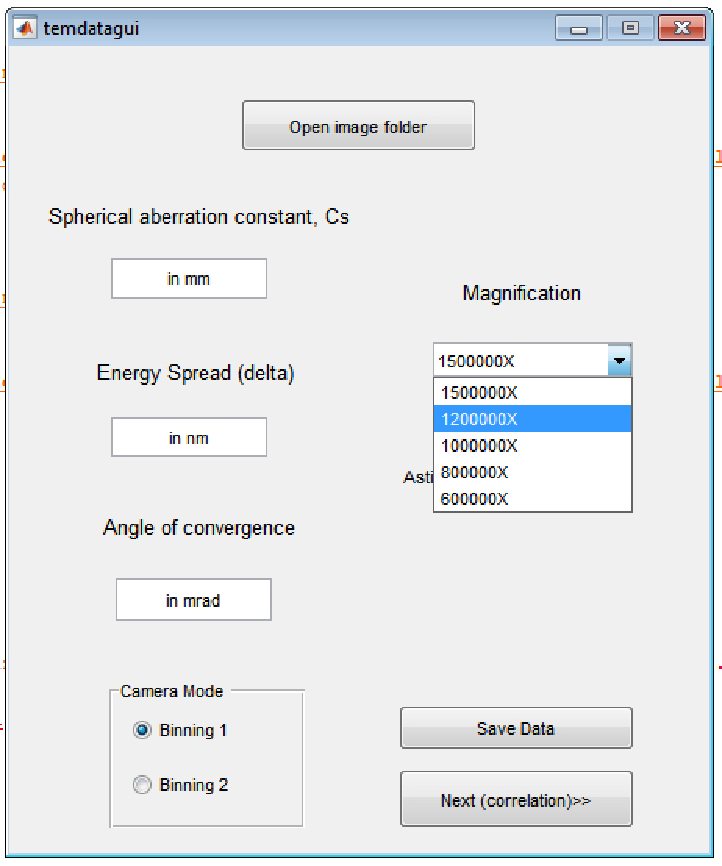
\includegraphics[width=0.6\textwidth]{figures/temdatagui.pdf}
    \caption{GUI window for acquiring initial parameters}
    \label{fig:temdatagui}
\end{figure}

Here all required data fields are to be filled, binning 2 mode is provided as a shortcut to reduce all calibration by a factor of two, as binning two images sometimes provides better signal to noise ratio.
All magnification values are calibrated for JEOL JEM 2100F at Chemical Sciences Devision, IISc, to customize it, provide own calibration value for each magnification in \texttt{switch} statement in \texttt{temdatagui.m} file at line 70.

Once all fields are filled, click on \textit{Open image folder} button, and select the folder containing all the images.
All images shall be present in serial order.

To save the provided data for next time, click on \textit{Save data}/
Then for image alignment click on \textit{Next(correlation)}

\begin{figure}
    \centering
    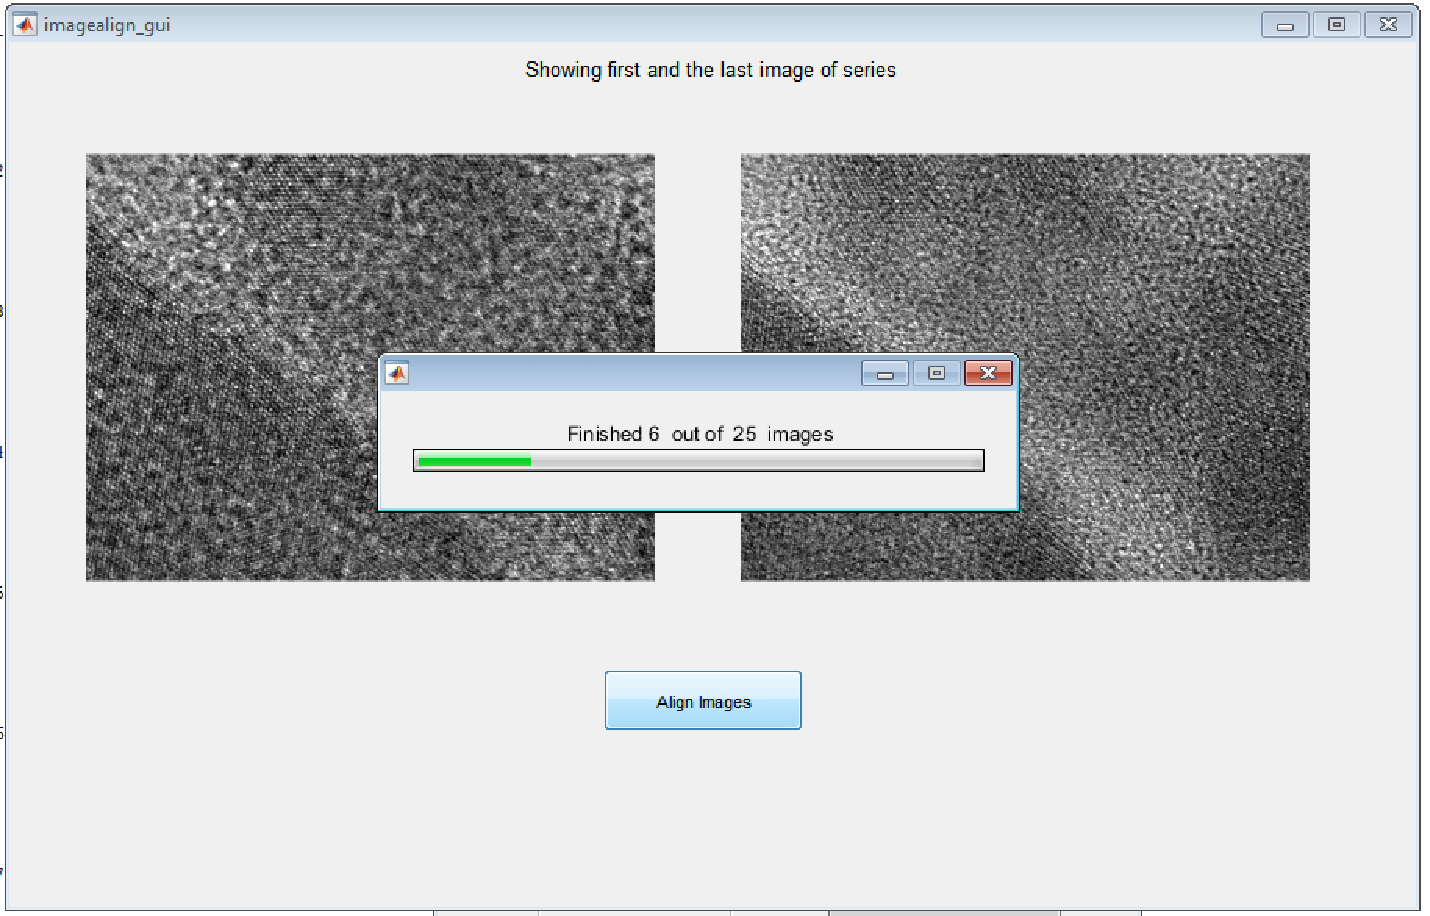
\includegraphics[width=0.6\textwidth]{figures/imalign.pdf}
    \caption{GUI window for aligning images}
    \label{fig:imalign}
\end{figure}

This shall open GUI for aligning images with display containing first and last image in the series.
Once `Align images' is clicked it shall ask the approximate defocus between 2 images (same can be achieved manually by \texttt{imgalign\_gui.m}).
Images are then propagated to that defocus value for better correlation estimation.\cite{meyer_symmetric}
After aligning images it will calculate FFT (using \texttt{fft\_profiler.m} file) for each image and shall present the GUI for defocus estimation.

\begin{figure}
    \centering
    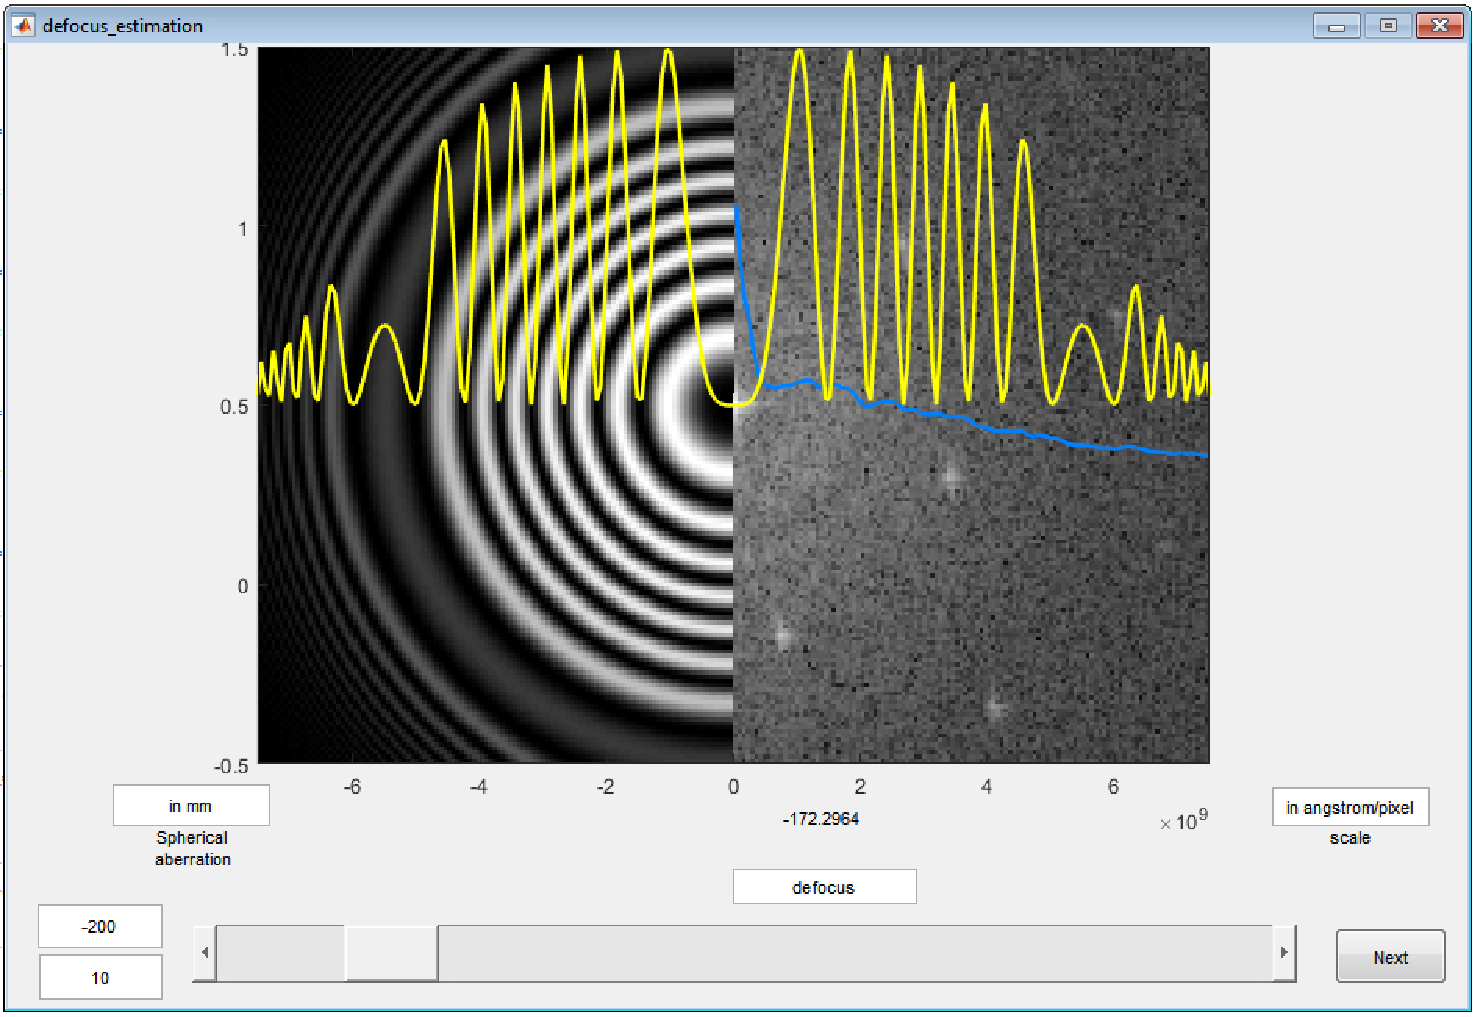
\includegraphics[width=0.6\textwidth]{figures/defocusgui.pdf}
    \caption{GUI window for estimating defocus}
    \label{fig:defocusest}
\end{figure}

Defocus estimation GUI (can also be launched manually by \texttt{defocus\_estimation.m}) will provide two input boxes on left bottom to give custom defocus range.
This serve as a smooth/coarse setting for slider as well.
You can edit lower bound and upper bound for the defocus slider and slider will accordingly adjust its values.
Current defocus value is displayed below the display window (-172.29 nm in current snapshot).
To go to any specific defocus value, enter the defocus value in defocus input box in the middle.
Spherical aberration and magnification can be changes here as well for better fit, but should be avoided.

Once defocus is estimated by matching minima of simulated CTF function (yellow curve) to the minima of acquired data (blue curve), press next to move to next image in series.
Once all images are done you shall be provided with calculated phase and amplitude.
All these results shall be saved in a \textit{'../usr\_data} folder as \texttt{*.mat} file which can be loaded later on for further processing if required.

Limitation: Modulus transfer function has to be calculated by \texttt{MTFestimate.p} program, which due to licensing agreement, cannot be included in current codes.\cite{VandenBroek2012}
Hence user has to obtain it on own and generate MTF file, name it as \texttt{MTF\_2d.mat} and keep it in \textit{../common\_data} folder.
This file is required by \texttt{gen\_mtf.m} function.

    \bibliography{references}
\end{document}